\documentclass[a4paper,12pt,twoside]{kth-mag}

\usepackage[T1]{fontenc}
\usepackage{helvet}
\usepackage{fourier}
%\usepackage{titlesec}
\usepackage{lipsum}
\usepackage[english,ngerman]{babel}%languages
\usepackage{textcomp}
\usepackage{modifications}
\usepackage{expdlist}
\usepackage{empheq}
\usepackage[usenames,dvipsnames]{xcolor}
\usepackage{booktabs}
\usepackage{multirow}
\usepackage{listings}
\makeatletter
\let\c@lofdepth\relax
\let\c@lotdepth\relax
\makeatother

%% main packages
\usepackage{amsmath,amsfonts,amssymb,amsthm}%math packages
\usepackage{siunitx}
%%\numberwithin{equation}{section}
\usepackage{graphicx,psfrag,color,subfig}
\usepackage{enumerate}%enumerated list
\usepackage{booktabs}%nice tables

%tikz, define its settings
\usepackage{pgf,pgfplots,tikz}
\usetikzlibrary{arrows,automata,plotmarks}
\usetikzlibrary{positioning}
\tikzset{
    state/.style={
           rectangle,
           rounded corners,
           draw=black,
           minimum height=1em,
           inner sep=1em,
           text centered,
           },
}


%%
%% Julia definition (c) 2014 Jubobs
%%
\lstdefinelanguage{Julia}%
{morekeywords={abstract,break,case,catch,const,continue,do,else,elseif,%
		end,export,false,for,function,immutable,import,importall,if,in,%
		macro,module,otherwise,quote,return,switch,true,try,type,typealias,%
		using,while},%
	sensitive=true,%
	alsoother={$},%
	morecomment=[l]\#,%
	morecomment=[n]{\#=}{=\#},%
	morestring=[s]{"}{"},%
	morestring=[m]{'}{'},%
}[keywords,comments,strings]%

\lstset{%
	language         = Julia,
	basicstyle       = \ttfamily,
	keywordstyle     = \bfseries\color{blue},
	stringstyle      = \color{magenta},
	commentstyle     = \color{ForestGreen},
	showstringspaces = false,
}
%% Definitions of additional environments
\newtheorem{definition}{Definition}
\newtheorem{theorem}{Theorem}
\newtheorem{lemma}{Lemma}
\newtheorem{corollary}{Corollary}
\newtheorem{remark}{Remark}
\newtheorem{proposition}{Proposition}
\newtheorem*{notation}{Notation}
\newtheorem*{example}{Example}
\newtheorem*{assumption}{Assumptions}

\DeclareMathOperator{\diag}{diag}
\DeclareSIUnit{\hour}{h} 

\usepackage{hyperref}
		\hypersetup{%
		bookmarksopen,
		bookmarksopenlevel={1},
		bookmarksnumbered,
		pdftitle = {Iterative learning control in prosumer-based DC microgrids},
		pdfsubject = {Bachelor thesis},
		pdfauthor = {Paraskevi Vorropoulou},
		pdfkeywords =  {hybrid systems, discrete event systems, abstractions, approximations},
		colorlinks,
		citecolor=black,
		linkcolor=black}
		
\title{Iterative learning control in prosumer-based DC microgrids}

\subtitle{Bachelor thesis}

\author{Paraskevi Vorropoulou}

\begin{document}

\frontmatter
\pagestyle{plain}
\selectlanguage{ngerman}

\begin{titlingpage}
\begin{center}
\begin{figure}[ht]
\begin{center}
		
\includegraphics[width=0.2\textwidth]{logos/tu-logo.pdf}
	\label{fig:tulogo}
\end{center}
\end{figure}

\vspace*{3cm}
%\LARGE
\sffamily\huge{\textbf{Iterative learning control in prosumer-based DC microgrids}}\\[1\baselineskip]
\normalfont
\vspace*{1cm}
\large
Bachelor thesis\\[0.5\baselineskip]
from\\[0.5\baselineskip]
Paraskevi Vorropoulou\\[0.5\baselineskip]
\normalsize
born on\\[0.5\baselineskip]
04.05.1998 in Berlin, Germany\\[0.5\baselineskip]
\vspace*{1cm}
02. November 2020
\vspace*{1cm}
\begin{table}[hb]
\begin{tabular}{ll}

Supervisor: & Lia Strenge\\
 & \\
Examiner: & Prof. Dr.-Ing. J\"org Raisch\\
& Control Systems Group\\
&  Institute of Energy and Automation Technology\\
& Faculty IV - Electrical Engineering and Computer Science\\
& Technische Universit\"at Berlin
\end{tabular}
\end{table}
 %%Datum der Abgabe - am besten selbst reinschreiben.

\end{center}

\end{titlingpage}

\clearpage

\begin{declarationoforiginality}

Hiermit erkläre ich, dass ich die vorliegende Arbeit selbstst\"andig und eigenh\"andig sowie
ohne unerlaubte fremde Hilfe und ausschließlich unter Verwendung der aufgef\"uhrten Quellen
und Hilfsmittel angefertigt habe.

\vspace{20mm}

Berlin, den \today \\

\vspace{10mm}
.................................................

\vspace{2mm}
Paraskevi Vorropoulou
\newpage
\end{declarationoforiginality}

\begin{zusammenfassung}
Seit Ende des 20. Jahrhunderts ist der Begriff der Energiewende von großer Bedeutung. Darunter versteht man den Übergang von fossilen Energieträgern zur nachhaltigen Energieressourcen, die immer häufiger Anwendung finden in der Stromerzeugung. Immer beliebter wird unter anderem die dezentrale Energieversorgung, die verbrauchernahe Erzeugung elektrischer Energie, sodass der Strombedarf unmittelbar für den Verbraucher gedeckt ist. Dazu zählen Inselnetze beispielsweise, die prosumer-basierend sind, also produzierend und verbrauchend gleichzeitig. 
\\Die zunehmende Nutzung von gleichstrom-basierend Ressourcen und Lasten ist auch ein Resultat der Energiewende, zum Beispiel die Photovoltaik und ist auch aus diesem Grund eine sehr relevante Lösung für die Elektrifizierung und verteilten Netzen im Niederspannungsbereich. 
\\Lastprofile in Energienetzen haben aber oftmals periodische Komponenten. Diese können durch geeignete Regelung gelernt und allzu ganz kompensiert werden, sodass auch gleichzeitig Regelungsenergie eines Systems gespart wird.  
Geeignet dafür ist die iterativ lernende Regelung (ILR). 
\\In dieser Arbeit wurde die iterative lernende Regelung 
in prosumer-basierenden Gleichstrominselnetzen angewandt, um die oben erwähnte Anforderung der Ausgleichung von periodischen Komponenten und des Energiesparens zu untersuchen. Dazu wird ein Modell für diese Art der Inselnetze vorgeschlagen und beschrieben mit geeigneten Gleichungen und Systemparametern als eine Ebene, und als weitere Kontrollebene wird die ILR damit verbunden, sodass ein Framework eingeführt wird. Dieses wird anschließend simuliert und dessen Leistung validiert. 
 
{\textbf{Schl\"usselw\"orter:} Prosumer-basiertes Inselnetz, Gleichstrominselnetz iterativ lernende Regelung, Dezentrale Energieversorgung, ...}

\end{zusammenfassung}

\selectlanguage{english}

\begin{abstracti}
Since the end of the 20th century, the concept of the energy transition has been of great importance. This is understood to mean the transition from fossil fuels to renewable energy resources, which are increasingly being used in power generation. Among other things, decentralized energy supply, the generation of electrical energy close to the consumer so that the electricity demand is covered directly for the consumer, is becoming increaslingly popular. This includes island networks, that are e.g. prosumer-based, i.e. producing and consuming simultaneously.
\\The increasing use of direct-current based resources and loads is also a result of the energy transition, and for this reason it is also a very relevant solution for electrification and distributed networks in the low-voltage range.
\\Load profiles in energy networks often have periodic components. These can be learned and compensated by appropriate controlling, so that the control energy of a system can be saved at the same time. The iterative learning control (ILC) is suitable for this purpose.  
\\ In this thesis the ILC is applied in prosumer-based direct current microgrids to investigate the above-mentioned requirement of balancing periodic components and energy saving. For this purpose, a model for this type of microgrids is proposed and described with suitable equations and system parameters as one level, and as a further control level the ILC is connected to it, so that a framework is introduced. This framework will then be simulated and its performance validated.

{\textbf{Keywords:} Prosumer-based microgrids, direct current microgrids, iterative learning control, distributed energy generation, ...}
\end{abstracti}

\begin{acknowledgements}

First, I would like to express my deep gratitude to M.Sc. Lia Strenge for her outstanding supervision and the support during the process of this work; Dr.Chris Rackauckas for the helpful comments in Julia programming.  \\ Furthermore many thanks for the love and energy from my parents, sisters, friends and my boyfriend. 
\vspace{10mm}

Paraskevi Vorropoulou

\end{acknowledgements}
\pagenumbering{arabic}
\clearpage
\tableofcontents
\clearpage
\listoffigures
\clearpage
\listoftables

\setlength{\parskip}{\baselineskip}
\setlength{\parindent}{0pt}

\mainmatter

%\pagestyle{newchap}

\chapter{Introduction}
\label{ch:intro}
%%%%%%%%%%%%%%%%%%%%%%%%%%%%%%%%%%%%%%%%%%%%%%%%%%%%%%%%%%%%%%%%%%%%%%%%%%%%%%%%%%%%%%%%%%%%%%%%%%%%%%%%%%%%%%%%%%%%%%%%%%%
In this chapter, we introduce the background and motivation for this thesis in Section \ref{sec:motivation} and the related work in Section \ref{sec:relatedwork}. Subsequently, a preview of all chapters in this thesis is given in Section \ref{sec:outline}. 

\section{Background and motivation}
\label{sec:motivation}
Microgrids have become one of the most popular research topics since the energy transition towards renewable energy and distributed generation. The centralized power system with fossil fuels is being transformed into a increasingly more decentralized power system including fluctuating renewable energy resources \cite{xiaohan_master}. Due to the increased use of direct current based loads and distributed power generation (e.g. photovoltaic) direct current microgrids are a very relevant and popular solution in low-voltage distribution grids with a fair power-sharing for all consumers. To achieve this, power sharing of the prosumer nodes of a direct current microgrid and bounded voltage deviation from the reference voltage of the grid must be assumed \cite{lia_master} by applying a lower-layer control with these objectives. 
\\However, the demand profiles in power grids contain periodic components.
Therefore, the iterative learning control is applied as a higher-layer controller to learn the daily periodicity in order to compensate the periodic demand patterns and reduce the decentralized lower layer control energy, since it is assumed that planned day-ahead power infeed is cheaper than instantaneous control power \cite{paperilc,xiaohan_master}. By learning the previous cycle, the iterative learning controller can optimize the performance of the system and reduce the error which is based on the previous cycle.
\\In this thesis, the overall network modeling of the direct current prosumer-based microgrid in a differential-algebraic equation framework is firstly proposed with the lower-layer control energy design based on the previously mentioned control objectives.
Furthermore, ILC framework will be proposed as a higher-layer controller, completing a hierarchically controlled system (to cope with different time scales (seconds to days)). 
\section{Related work}
\label{sec:relatedwork}
In the field of power systems, \cite{Hatzi}, as well as \cite{microgrid_concept} and \cite{concept} define the main points of direct current microgrids.  \cite{lia_stability} offers us the concept of meshed DC microgrids, and \cite{lia_master} offers the concept of the droop controlled low-voltage DC microgrids. Both of them have the producer-consumer distinguishment and based on these equations the prosumer-model can be derived. Both sources by Lia Strenge provide differential-algebraic equations for the overall lower-layer microgrid satisfying the power sharing and bounded voltage deviation control objectives.
\\For the control methods of direct current microgrids, the multilayered schema is explained in \cite{controldc} and \cite{hier_control} and \cite{controldc_energy_man} offer contributions on the two-layer control. 
\\The concepts of iterative learning control are proposed by Moore in \cite{moore_ilc} and \cite{vl_ilc} with Fig. \ref{fig:figure_ILC}. Obviously this work is based on the previous work of \cite{paperilc}, that provides an overall hierarchical control model for a prosumer-based alternating current microgrid with iterative learning control.


\section{Outline}
\label{sec:outline}
This work is divided as follows:
\begin{itemize}
\item \textbf{Chapter 1}: An introduction to the motivation, background and related work to this thesis
\item \textbf{Chapter 2}: An overview of the theoretical preliminaries of the prosumer-based DC microgrids, power network modeling and the two-layer control with the ILC method for a better understanding of the following context 
\item \textbf{Chapter 3}: The proposal of the prosumer-based DC microgrid network model, based on the producer-consumer microgrid model, followed by the representation of the ILC design
\item \textbf{Chapter 4}: The simulations of the overall model, a list of the results, the model validation and interpretation
\item \textbf{Chapter 5}: Summary and future directions
\end{itemize}




\chapter{Theory and background information}
\label{ch:theo}
\par Now, that the topic of the thesis was introduced and the question of the research was stated, there are necessary preliminaries that need to be mentioned and explained, in order have a better understanding fpr the following chapters. \\ Thus, we will clarify the basics of the \textit{microgrids} and in particular the \textit{(prosumer-based) DC microgrids} (\ref{sec:dcmicrogrids}), \textit{power network modeling} (\ref{sec:power_network})and the \textit{iterative learning control} method (\ref{sec:ilc})
 
\section{Basics of prosumer-based DC microgrids}
\label{sec:dcmicrogrids}
\par In this section we are going to introduce the (prosumer-based DC) microgrid concept. Firstly, in order to understand the functionality of the microgrids and especially the DC microgrids, which are going to be introduced later, we should discuss, what \textit{Distributed generation} is.
\subsection{Distributed generation}
\label{subsec:der}
Distributed generation is the electrical generation and storage performed by a variety of small, grid-connected or distribution system-connected devices referred to as distributed energy resources (\textit{DER}), as defined in \cite{dg_wiki}. DER systems typically use renewable energy sources such as e.g. biogas, fuel cells, solar power or wind power \cite{dg_wiki}. Different from a transmission network, distributed generation basically generates electricity close to the consumer, which means that the efficiency of the current generation plant usually only covers the energy demand of current consumers that are directly next or in the closer environment.
\\Another difference between distributed and the central generation, as described in \cite{epa_dg} is, that the distributed resources work with low voltages, with the central generators are provided through the higher voltages. Therefore, distributed generation can reduce electricity losses along transmission and distribution lines when connected to the electric utility’s lower voltage distribution lines \cite{epa_dg}. It can also provide lower-cost electricity and higher power reliability and security with fewer environmental consequences such in the common power generators. 
\\Distributed generation can be a single structure, such as a home or a place of residence, or it may be part of a \textit{microgrid}, such as a large college campus or a industrial plant \cite{dg_wiki}. \par Since the operation area of a microgrid is now clarified, we will introduce in the next subsection with the microgrid and in particular the DC microgrid.
\subsection{ Microgrids}
\label{subsec:microgr}
\begin{figure}[h]
\begin{center}
    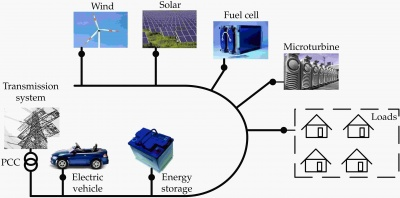
\includegraphics[scale=0.8]{pictures/microgrid_concept.jpg}
    \caption{The microgrid concept}
    \label{figure_microgrid_concept}
\end{center}
\end{figure}
In this scope we are going to use the definition of a microgrid as in \cite{Hatzi}.
\begin{definition} from \cite{Hatzi} \\
"Microgrids comprise LV distribution systems with [...] DER (microturbines, fuel cells, PV, etc.) together with storage devices (flywheels, energy capacitors and
batteries) and flexible loads. Such systems can be operated in a non-autonomous way, if
interconnected to the grid, or in an autonomous way, if disconnected from the main grid. The
operation of microsources in the network can provide distinct benefits to the overall system
performance, if managed and coordinated efficiently."
\end{definition}
By this definition we understand that a microgrid consists of a limited number of generation units, storage units and demand resources, all together located in a local distribution grid, as sketched in \ref{figure_microgrid_concept} \cite{microgrid_concept}. Microgrids do not always have a synchronous connection to the main generation net which means that the tasks that are necessary for a constant and safe operation need to be provided, in cases of emergency \cite{concept}. They should though have the option of a synchronous connection to the main generation network. Such systems arise from the geographical circumstances that make a connection to the main network costly and almost impossible. Microgrids on the other hand serve to an increased security of supply, should a collaps of the main network occur \cite{concept}.\\ An introduction on the alternating and direct current microgrids is given in the next section. Since the main focus of this thesis is on the direct current type of microgrids, the alternating current will be only mentioned summarized.  
\subsection{Direct current versus alternating current microgrids}
\label{subsec:acdc}
\par Electric charge in \textit{alternating current} (AC) changes direction periodically and is characterized by an amplitude and a frequency. The electric charge in \textit{direct current} (DC) on the other hand only flows in one direction and remains constant the whole time. Back in time, DC could not be easily converted to high voltages due to the high transformation losses. Therefore, AC is the preferred type of current for power networks and used until today \cite{mikieus}, but with the development of the DC-based power electronics for generating as well as load that allow efficient voltage transformation, DC is on the rise again and more often used in microgrids.
\\ In \cite{versus}, Table 4 in [25, p.399] a comparison between AC and DC microgrids is given. Since the line losses (the power that is lost in a conductor during transmission and distribution phase, as in \cite{lineloss}) in AC distribution are high, it leads to less efficiency and less power transmission. In DC distribution the power transmission is more efficient due to a lower line loss, no reactance in the line and a low line resistance itself. DC distribution does not obviously require frequency monitoring, since the frequency of DC is constantly zero, has no electromagnetic interference, like AC distribution does and is easier when it comes to the analysis, since only real numbers are involved. \\
Hence, DC distribution is chosen in this work due to higher efficiency and lower line losses. Finally, prosumer-based DC microgrid is defined in the next section.
\subsection{Prosumer-based (DC) microgrids}
\label{subsec:prosumer}
\par In \ref{subsec:der}, it is mentioned that " [...] distributed generation basically generates electricity close to the consumer [...]". Obviously there is a distinction between generation and consumption for the energy transfer. The DC microgrid model, as introduced in \ref{subsec:microgr} is also based on the separation of the as called \textit{producers} and \textit{consumers}. By definition:
\begin{itemize}
    \item A distribution unit is called \textit{producer}, if it feeds power into the grid. 
    \item The distribution is called \textit{consumer} when it draws power from the grid.
\end{itemize}
\par As in \ref{subsec:der} producers "[...] typically (are) [...] renewable energy sources such as e.g. biogas, fuel cells, solar power or wind power that can feed power into the grid. Consumers are power loads such as homes or places of residence that draw the power from the grid for each purpose. 
\\Spurred by technology development and regulatory frameworks, self-consumption of distributed
renewable electricity generation has gained relevance in many power markets around the world \cite{prosumage}. But also in a daily usage, consumers can draw electricity at the same time and, for example, produce it via the solar photovoltaic panels on the roof and feed it into the grid.
\\For our research we need to understand the definition of a \textit{prosumer}. The word is a portmanteau \cite{portm} , a linguistic blend of the words producer and consumer. Prosumers are units which produce energy and feed it into a distribution network, like in the solar photovoltaic panels for example \cite{prosume}. They feed power into the grid in case that the produced energy is bigger than the energy demand. Prosumer draw the same power from the grid, when the energy demand exceeds the production of it. %\noindent
\\Using this information in our DC microgrid model mentioned in section \ref{subsec:acdc}, the following definition \ref{prosumer_def} for prosumer-based DC microgrids can be given. \\

\begin{definition}
\label{prosumer_def}
A prosumer-based microgrid is a power network where every node of the grid can be a producer, a consumer or idle. In other works every node can feed power into the grid, draw power from the grid or not participate in the grid.
\\Every node $\alpha \in \mathcal{N}$ can feed power $P_{\alpha} \in \mathbb{R}_{\geq 0}$ into the microgrid with $P_{\alpha} \geq 0 $, receive power from the microgrid with $P_{\alpha} \leq 0 $ or not participate in the microgrid.
\end{definition}
Since the prosumers are described as \textit{nodes}, in the next section we are going to introduce the basics of power network modeling as in graph theory, so that we have a better overview for the modeling of  prosumer-based DC microgrids in Section \ref{sec:model}
\section{Basics of power network modeling}
\label{sec:power_network}
\begin{figure}[h]
\centering
    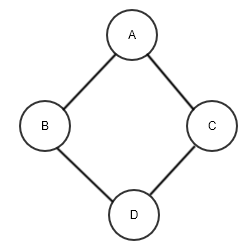
\includegraphics[scale=0.8]{pictures/undirected_graph.png}
    \caption{An example of an undirected graph}
    \label{graph}
\end{figure}
\par A simple power network can be represented as a graph $\mathcal{G}:=(\mathcal{V},\mathcal{E})$, where $\mathcal{V} \in \mathbb{N}$ is the set of \textit{vertices} or \textit{nodes} and $\mathcal{E} \subseteq (\mathcal{V} \times \mathcal{V})$ the set of \textit{edges} \cite{graph_theory}. The nodes are connected via the edges and we consider the connection as \textit{undirected}. In graph theory, a node is considered \textit{incident} to an edge if the node is one of the two node the edge connects. An example of an undirected graph is shown in \ref{graph} \cite{un_graph}. 
\\As described in Definition \ref{prosumer_def}, a node from a power network in the form of a graph is a representation of a prosumer, so either a producer, consumer or idle. An edge represents the power lines that connects the prosumers to each other. Current flows through the power lines, feeding or drawing electricity to or from the nodes. This means that the current flows in both direction, which is why the graph is also considered as \textit{undirected}. 
\\ Let $N \in \mathbb{N}$ be the number of prosumers in a DC microgrid connected to each other. The prosumers are at grid nodes $j,k \in \{1,2,..,N\} =: \mathcal{N} \subset \mathbb{N}$. Then the number of the edges or \textit{number of power lines} is defined as \cite{lia_master}: 
\begin{align*}
    m &\leq \frac{N(N-1)}{2}
\end{align*}
The index $h \in \{1,2,..,m\} =: \mathcal{M} \subset \mathbb{N}$ is then used for the power lines \cite{lia_master}. The connection $jk$ is incident with the grid nodes $j$ and $k$ and starts from node $j$ to node $k$. It contains the power line $h$. \\To describe the relationship between between nodes and power, we use the \textit{incidence matrix} $\boldsymbol{M}$ of a network graph with the dimension $m \times N$ with 
\begin{align}
\label{equation:incidence_def}
    \boldsymbol{M} &= \begin{bmatrix} m_{1,1} & \dots & m_{1,N} \\ \vdots & \ddots& \vdots \\ m_{m,1} & \dots & m_{m,N} \end{bmatrix} \in \mathbb{R}^{m \times N}
\end{align}
where the entries for each connection are $m_{h,j} = 1$ and $m_{h,k} = -1$. All other entries $m_{h,\kappa}=0$ are the non-incident nodes $\kappa \in \mathcal{N}$ to the power line h \cite{lia_master}. \\ With the incidence matrix $\boldsymbol{M}$, the network topology is uniquely described. By using the incidence matrix, we can describe the Kirchhoff Laws in the network as constraints \cite{lia_master}. Since the topic of this thesis is to control the overall model of the prosumer-based direct current microgrid with the iterative learning control method, the next section introduces the two-layer control with the iterative learning control method.
\section{The two-layer control with the iterative learning control method}
\label{sec:ilc}
In this section, we get to know the basics of the two-layer control with the \textit{iterative learning control method}, by introducing in \ref{subsec:feedback} the \textit{standard control feedback loop}, which is the base for many control applications. We will later delve into the \textit{low-layer-control} and the \textit{high-layer-control}, that result the \textit{two-layer-control method} (\ref{subsec:twolayer}), one specialization of which is the iterative learning control (\ref{subsec:ilc}).
%Seite 170 - Iterative Learning control 
\subsection{Basics of of the standard control feedback loop}
\label{subsec:feedback}
\begin{figure}[h]
\centering
    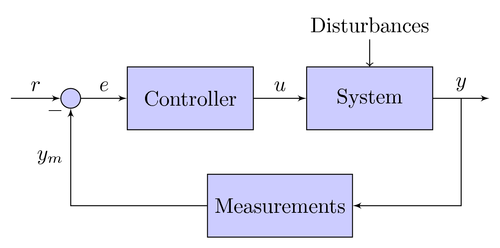
\includegraphics[scale=0.5]{pictures/control-system-principles.png}
    \caption{Closed-loop model in standard feedback control loop block representation \cite{cs_princi}, with the definitions as in \cite{cs_princi_wiki,lia_master} $r$ for the reference, $e$ for the measured error, $u$ for the system input, $y$ for the system output and $y_m$ for the measured system output}
    \label{clm_standard_feed}
\end{figure}
In engineering, processes in form of a dynamical (time-dependent) system need to be controlled, in order to achieve control stability and an optimal behavior. Therefore, a \textit{controller} is designed uniquely for the to-be-controlled system, to automatically regulate the output and keep it within the systems desired input value or “set point” \cite{oploop}. If the system input changes for whatever reason, the output of the system must respond accordingly and change itself to reflect the new input value \cite{oploop}. 
\\In most systems the controlling process, the controllers actions depend on the feedback from the process. In other words, we can control a process by adding an amount of the output to the measured error, so the actual output is compared with the desired and the error can be reduced or even eliminated. 
This type of control system is called \textit{closed-loop control system} or \textit{feedback control system} and two-layer controllers belong to this family of controls. \\The basics of the \textit{two-layer control method}, which is going to be used in this research, are going to be explained in the next section \ref{subsec:twolayer}.
\subsection{Two-layer control}
\label{subsec:twolayer}
Microgrids control and management are, not as in the standard feedback control loop described in section \ref{subsec:feedback}, usually divided in multiobject tasks, covering mostly different time scales and physical levels \cite{controldc}. This schema is divided hierarchically and every layer has a different task from e.g. frequency control to energy management. Two-layer architectures, which are used in our research as control architecture are e.g. used among others for economic optimization \cite{hier_control}.\\
As described in \cite{paperilc}, in microgrids, hierarchical control is
typically divided in \textit{primary}, \textit{secondary} and \textit{tertiary control}, also called energy management, referring to the same
tasks. In particular it is said that "[...] \textit{primary control is responsible for fast frequency
stabilization and reacts in seconds, secondary control restores the frequency to its setpoint in terms of minutes
and tertiary control refers to economic dispatch questions
in the time scale of hours and days[...]}" \cite{paperilc}. The definition is referring to systems, where frequency is a control property. Since in direct current microgrids no frequency appears, primary, secondary and tertiary control, proposed by Meng and Ferrai Trecate in \cite{controldc} and Luis Orlando Polanco Vasquez et al. in \cite{controldc_energy_man} are considered as follows: 
\begin{enumerate}
    \item \textit{Primary control} performs the control of local power,
    voltage, and current. It normally follows the set-points
    given by upper level controllers and is communication-less power sharing among DERs \cite{controldc}. 
    \item \textit{Secondary control} appears on top of primary control.
    It deals with issues in the system level, such as power quality regulation, microgrid synchronization with external grid for smooth reconnection [...] and so on \cite{controldc}.
    \item \textit{Tertiary control} is issued with optimization, management, and overall system regulations \cite{controldc}. It considers the economical concerns [...] and manages the power flow between the microgrid and the main grid \cite{controldc_energy_man}.
\end{enumerate}
In decentralized hierarchical control, regulation takes place with only local information \cite{controldc_energy_man} and the control functions can be distributed into local controllers, or in our case \textit{lower-layer controllers} and upper-level or \textit{higher-layer controllers}. Primary and secondary control can be combined as the lower-layer control and tertiary control as the higher-layer control. The grid itself and the low-level controller form the \textit{compound plant} Placing the higher-layer controller into the system can save lower-layer control energy \cite{paperilc}. \\ In this research, the two-layer schema is used with an \textit{iterative learning controller} as a higher-layer controller, proposed by Strenge et al. in \cite{paperilc}. The iterative learning method is going to be introduced in the next section.
\subsection{Iterative learning control}
\label{subsec:ilc}
\begin{figure}[h]
	\centering
	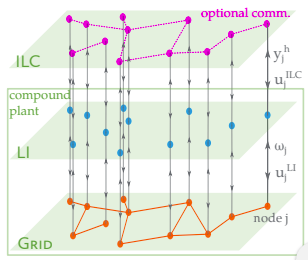
\includegraphics[scale=0.7]{pictures/control_hierarchy.png}
	\caption{Control hierarchy with low-level control (LI) and iterative learning controller (ILC) \cite{paperilc}. Here, the grid current is alternating and the control achievement is the bounded frequency deviation ($\omega_j$)}
	\label{fig:control_hier}
\end{figure}
The \textit{iterative learning control} (ILC) is a method that addresses the problem of transient response performance for systems that operate in a repetitive mode \cite{vl_ilc}. Based on the errors observed during past operations, the transient response is improved by adjusting the input to the plant during future \cite{vl_ilc}.
\begin{figure}[h]
\centering
    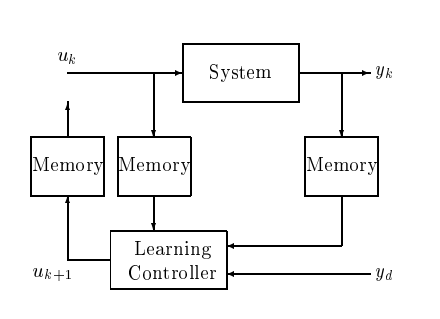
\includegraphics[scale=0.56]{pictures/ILC_schema.png}
    \caption{Iterative learning control configuration}
    \label{fig:figure_ILC}
\end{figure}
The basic idea of iterative learning control is illustrated in Figure \ref{fig:figure_ILC} \cite[p.427]{moore_ilc}. The ILC algorithm has the form, proposed by \cite{paperilc}
\begin{align}
    u^{c+1}= u^{c}- Ly^{c}
\end{align}
The power $c$ is the cycle number. In this work $c$ has the duration of one day. During the $c$-th repetition $u^c$ is inputted, producing an output $y^c$. While the input and output is memorized, this output is observed as an error and based on this the next input $u^{c+1}$ is modified. The new input is designed so that the new error is smaller than the previous input. By time shifting we get
\begin{align}
    u^{c}= u^{c-1}- Ly^{c-1} \label{eq:ilc_inp_th}
\end{align}
with $L$ a single scalar parameter $ L = \kappa \in \mathbb{R}_{>0}$.\\
The proposed ILC approach is applied to learn a power infeed that compensates the periodic demand component and to save lower-layer-energy \cite{paperilc}. \\Now that the basics of prosumer-based direct current microgrids and the iterative learning control have been introduced, in the next chapter the network dynamics with the lower-layer and higher-layer controller can be modeled.


\chapter{Network modeling of the prosumer-based DC Microgrid and the iterative learning controller design}
\label{sec:model}
After having explained the research work and summarized the necessary theory preliminaries in the previous chapters, this chapter goes through the steps of modeling the prosumer-based direct current microgrid with iterative learning control. Section \ref{sec:networkmodel} starts off with the \textit{low voltage direct current microgrid dynamics} (\ref{subsec:prod_cons_model}), followed by the definition of the \textit{prosumer-based direct current microgrid model} (\ref{subsec:prosumer}). The following section \ref{sec:ilc} derives the \textit{structure and design of the iterative learning controller}, by defining the \textit{control objectives} (\ref{subsec:conobj}), the structure of the \textit{higher-layer controller} (\ref{subsec:hlc}) and the \textit{learning dynamics} (\ref{subsec:learndyn}).

\section{Network model of the prosumer-based DC microgrid with lower-layer control}
\label{sec:networkmodel}
In this section, we model the network of the prosumer-based DC microgrid and define the dynamics of it. The model is adapted by the \textit{low voltage direct current microgrid} dynamics, proposed by Lia Strenge in her master thesis \cite{lia_master}, where a distinction is made between producers and consumers. In this thesis, however, the model and equations are adapted to combine producer and consumer as prosumer. Despite everything it is necessary to be introduced to these dynamics, to have a better understanding for the modeling in Section \ref{subsec:prosumermodel}

\subsection{Network modeling of the producer-consumer DC microgrid}
\label{subsec:prod_cons_model}
This Section serves as a base and defines the equations, that inspired the prosumer-based microgrid network dynamics and the lower-layer controller, respectively, with no influence of the ILC. We assume a constant demand for the consumer nodes and no higher-layer control input, to make the derivation of the equations clearer. \\
As explained above, the modeling of this network topology and the definitions and equations mentioned in this Section are proposed by Lia Strenge in "\textit{Modeling and simulation of a droop controlled swarm
type low voltage DC microgrid in a DAE framework - Master Thesis}" \cite{lia_master}, as well as the work "\textit{Stability of meshed DC microgrids using
probabilistic analysis}" by L. Strenge, H. Kirchhoff, G.L. Ndow and F. Hellmann \cite{lia_stability}.
\\ Recall from \ref{sec:power_network}, that a microgrid is considered as an \textit{undirected graph}. Then $N \in \mathbb{N}$ is the number of producers and consumers. The grid nodes $gn \in \{1,2,...,N\} =: \mathcal{N} \subset \mathbb{N}$ with = $\mathcal{N} = \mathcal{N}_P \cup \mathcal{N}_C$ represent the producers $n_P \in \mathcal{N}_P$ with index $j = 1,...,n_P$  and consumers $n_C \in \mathcal{N}_C$ with index $k = n_P+1,...,N$ and $n_P + n_C = N$, while the edges $pl \in \{1,2,...,m\} =: \mathcal{M} \subset \mathbb{N}$ with $m \leq N(N-1)/2$ and the index $jk$, represent the power lines connecting the producers with the consumers. 
\\ The network is modeled as an undirected connected graph with the edge-vertice-incidence matrix $\boldsymbol{M} \in \mathbb{R}^{m \times N }$, see (Eq. \ref{equation:incidence_def}) in Section \ref{sec:power_network}. Since the network is electric, the Kirchhoff laws must hold. The currents sum to zero at each node (Kirchhoff current law) and the voltages sum to zero in each mesh (kirchhoff voltage law) \cite{lia_master}. With these laws, we obtain the equations \cite{lia_master}:
\setlength{\abovedisplayskip}{5pt}
\setlength{\belowdisplayskip}{5pt}
\setlength{\abovedisplayshortskip}{0pt}
\setlength{\belowdisplayshortskip}{0pt}
\begin{align}
    v_{pl}(t) &= \boldsymbol{M}v_{gn}(t) \label{eq:incv} \\
    i_{gn}(t) &= \boldsymbol{M}i_{pl}(t) \label{eq:inci}
\end{align}
where $t \in \mathbb{R}$ is the time in seconds, $\boldsymbol{M} \in \mathbb{R}^{m \times N}$ is the incidence matrix of the network; $v_{pl}(t) = (v_{pl,1}(t),...,v_{pl,m}(t))^T: \mathbb{R} \rightarrow \mathbb{R}^m$ is the vector of power line voltages in volt or the voltage difference between the connected grid nodes, respectively; $v_{gn}(t) = (v_{1}(t),...,v_{N}(t))^T: \mathbb{R} \rightarrow \mathbb{R}^N$ is the vector of grid node voltages in volt; $i_{gn}(t) = (i_{1}(t),...,i_{N}(t))^T: \mathbb{R} \rightarrow \mathbb{R}^N$ is the vector of the currents sum at the grid nodes in ampere and $i_{pl}(t) =(i_{pl,1}(t),...,i_{pl,m}(t))^T: \mathbb{R} \rightarrow \mathbb{R}^m$ is the vector of the power line currents in ampere \cite{lia_master}. \\Furthermore, we make the following assumptions:
\begin{enumerate}[i.]
    \item Every node can feed electricity into the microgrid (producer with $i_{to,grid,j}(t) > 0, j = 1,...,n_P$), receive from the microgrid (consumer with $i_{to,grid,k}(t) < 0, k = n_P+1,...,N$) \cite{lia_stability} 
    \item At each node, there is no other information available other than local variables. Hence, the control is fully decentralized.
    \item The generation current at the producer nodes is known with \cite{lia_stability}
    \begin{align}
        i_{gen,j}(t) = K_{D,j}(V_{ref,j} - v_j(t)) \label{eq:i_gen}
    \end{align} where $K_{D,j} > 0$ is the voltage droop coefficient and $V_{ref,j}$ the reference voltage at producer node $j \in \mathcal{N}_P$. Droop control (with its according droop coefficient mathimatically) is applied in a microgrid to stabilize the voltage drop \cite{voltage_droop}. 
    \item The current to the load at the consumer nodes is assumed to be known with \cite{lia_stability}
    \begin{align}
        i_{load,k}(t) = \frac{P_k(t)}{v_k(t)}, v_k(t) \neq 0 \label{eq:i_load}
    \end{align} where $P_k$ is the load power drawn from the grid at consumer node $k \in \mathcal{N}_C$. 
    \item \label{ass:induct} A power line in low voltage direct current applications behaves mostly inductive \cite[p.28]{lia_master} with the context
    \begin{align}
        L_{pl,jk} \frac{di_{pl,jk}(t)}{dt} = v_{pl,jk}(t)-R_{pl,jk}i_{pl,jk}(t) \label{eq:induct}
    \end{align} where $L_{pl,jk}$ is the known inductance, $R_{pl,jk}$ the known resistance, $i_{pl,jk}(t)$ the power line current and $v_{pl,jk}(t)$ the power line voltage at power line $jk \in \mathcal{M}$. Since current flows in both directions, we further assume $L_{pl,jk} = L_{pl,kj}$, $R_{pl,jk} = R_{pl,kj}$, and $i_{pl,jk}(t) = i_{pl,kj}(t)$
    \item \label{item:cap} A producer or consumer can be electrically modeled by a current source, represented by the equation (Eq. \ref{cap_eq}) and a capacitor in parallel as in (Eq. \ref{cap_i}) \cite{lia_master}. 
    \begin{align}
        i_{gn}(t) &= f(t,q) - i_{cap}(t) \label{cap_eq}\\
        i_{cap}(t) &= \boldsymbol{C_{cap}}\frac{dv_{gn}(t)}{dt} \label{cap_i}
    \end{align}
    with $f: \mathbb{R}\times \{0,1\}^N \rightarrow \mathbb{R}^N$ as a source current vector in Ampere, $i_{cap}(t) = (i_{cap,1}(t),...,i_{cap,2}(t))^T: \mathbb{R} \rightarrow \mathbb{R}^N_{>0}$ as a vector of capacitor currents in Ampere and $\boldsymbol{C_{cap}} = \diag{(C_{cap,1},...,C_{cap,N})}^T \in \mathbb{R}^{N \times N}_{>0}$ as diagonal matrix of capacitances in Farad \cite{lia_master}.
\end{enumerate}
In assumption \ref{item:cap}. the source current vector can be distinguished between the generation current from (Eq. \ref{eq:i_gen}) and the load current from (Eq. \ref{eq:i_load}) with 
\begin{align}
    f(t,q) =\begin{cases}
K_{D,j}(V_{ref,j} - v_j(t)),& i_{to grid,i}(t) >0\\
\frac{P_k(t)}{v_k(t)}, & \, i_{to grid,i}(t) <0
\end{cases} \label{eq:fallunterscheidung_strom}
\end{align}
with $i = 1,...,n$ as the considered node and $v_k(t) \neq 0$. Furthermore we assume that the load power is constant, $P_k(t) = P, P \in \mathbb{R}$ Combining equations (Eq. \ref{eq:fallunterscheidung_strom}), (Eq. \ref{cap_eq}) and (Eq. \ref{cap_i}) and distinguishing between producer and consumer grid node voltage with 
\begin{align}
    v_{gn}(t) = \left[\begin{array}{c} v_P(t) \\ v_C(t) \end{array}\right] 
\end{align}
producers listed first ($v_P(t) = (v_1(t),...,v_{n_P}(t))^T$) and consumers listed last ($v_C(t) = (v_{n_P+1}(t),...,v_n(t))^T$), we get the following equation \cite{lia_stability}:
\begin{align}
    \boldsymbol{C_{cap}}\left[\begin{array}{c} \frac{dv_P(t)}{dt} \\ \frac{dv_C(t)}{dt} \end{array}\right] = -i_{gn}(t) + \left[\begin{array}{c} \boldsymbol{K_{D}}(V_{ref,P} - v_P(t)) \\ P/v_C(t) \end{array}\right]
\end{align}
$i_{gn}(t) = (i_{gn,1}(t),...,i_{gn,N}(t))^T: \mathbb{R} \rightarrow \mathbb{R}^N$ is the vector of the currents sum at the grid nodes in ampere; $\boldsymbol{K_D} = \diag(K_{D,j})$ is the diagonal droop coefficient matrix, $j$ the producer index, as above; $V_{ref,P} = (V_{ref,1},...,V_{ref,n_P})^T$ the vector of the reference node voltages of the producers; $P = (P_1,...,P_{n_c})^T$ is the load power vector of the consumers \cite{lia_stability}. \\From equation (Eq. \ref{eq:induct}) in assumption \ref{ass:induct} we get the equation: 
\begin{align}
    \boldsymbol{L_{pl}} \frac{di_{pl}(t)}{dt} = v_{pl}(t)-\boldsymbol{R_{pl}}i_{pl}(t) 
\end{align} in vector representation, with $\boldsymbol{L_{pl}} = \diag(L_{pl,jk})$ the diagonal power line inductance matrix and $\boldsymbol{R_{pl}} = \diag(R_{pl,jk})$ the diagonal power line resistance matrix \cite{lia_stability}. Recall, that $v_{pl}(t) = (v_{pl,1}(t),...,v_{pl,m}(t))^T: \mathbb{R} \rightarrow \mathbb{R}^m$ is the vector of power line voltages in volt or the voltage difference between the connected grid nodes.
\\With (Eq. \ref{eq:inci}) and (Eq. \ref{eq:incv}) we obtain the model equation system (Eq. \ref{eq:1}) and (Eq. \ref{eq:2}) in matrix vector form \cite{lia_stability}
\begin{align}
    \boldsymbol{L_{pl}} \frac{di_{pl}(t)}{dt} &= \boldsymbol{M}v_{gn}(t)-\boldsymbol{R_{pl}}i_{pl}(t) \label{eq:1} \\
    \boldsymbol{C_{cap}}\left[\begin{array}{c} \frac{dv_P(t)}{dt} \\ \frac{dv_C(t)}{dt} \end{array}\right] &= -\boldsymbol{M}i_{pl}(t) + \left[\begin{array}{c} \boldsymbol{K_{D}}(V_{ref,P} - v_P(t)) \\ P/v_C(t) \end{array}\right] \label{eq:2}
\end{align}
The overall producer-consumer direct current microgrid model is shown in Figure
 \ref{fig:prod-cons-micro}. 
%\label{subsec:prodconsmodel}
\begin{figure}[h]
\centering
    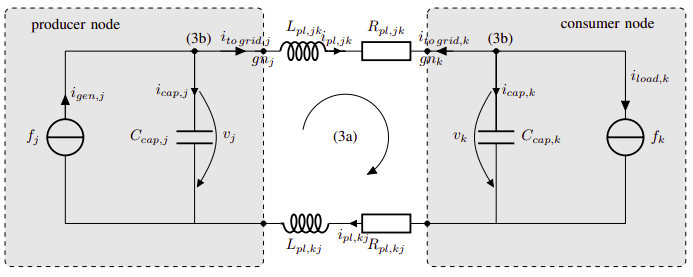
\includegraphics[scale=0.5]{pictures/prod-cons-microgrid.png}
    \caption{Model for the direct current microgrid. Here, simplified for $n = 2$ nodes and time argument $(t)$. Index $j$ for producers, index $k$ for consumers. $i_{gen,j}(t) = f_{j}(t)$ are droop controlled sources (Eq. \ref{eq:i_gen}), $i_{load,k}(t) = f_k(t)$ are constant power load (Eq. \ref{eq:i_load}) \cite{lia_stability}}
    \label{fig:prod-cons-micro}
\end{figure}
Based on this system we can now define the network model of the prosumer-based structured microgrid in the next Section.
Note that the load power is only in this Section considered as constant. Also, there is no higher-layer control input. For the purpose of the iterative learning control we must assume in the next Section that the power demand has a periodic and fluctuating character. 
\subsection{Network model of the prosumer-based DC microgrid with lower-layer control}
\label{subsec:prosumermodel}
\begin{figure}[h]
	\centering
	\caption{Model for the proposed prosumer-based direct current microgrid. Here, simplified for $n = 2$ nodes.}
	\label{fig:pros-micro}
\end{figure}
Based on the network modeled in Section \ref{subsec:prod_cons_model}, the slightly different prosumer-based direct current model can be derived in this Section. Additionally the low-level control input is going to be used as well as the high-level control input, since the low-layer control structure must be considered now. It is also now going to be assumed, that the load profiles have periodic components in contrast to Section \ref{subsec:prod_cons_model}. \\
In Section \ref{subsec:prosumer}, it is considered that a node in a prosumer-based dirrent current microgrid can feed power into the microgrid, receive power from it or not participate in the microgrid, see Definition \ref{prosumer_def}. Therefore there is no differentiation anymore between producer and consumer; A node must be modeled as one unit combined by the two at first seperate units. 
\\Recall Figure \ref{fig:prod-cons-micro}, where the model for the direct current, non-prosumer-based microgrid is illustrated. The seperate producer $j$ node is connected via the power line $jk$ with the consumer node $k$. For the prosumer-based model, this schema can be adapted, but the power line $jk$ connects prosumer $j$ with prosumer $k$, respectively. Furthermore, $N \in \mathcal{N}$ is the number of prosumers. Therefore, the grid node voltages are now defined as \\$v_gn(t) = (v_1(t),...,v_n(t))^T$.
Obviously, the node structure needs to be changed, so it can produce but also consume simultaneously.
\\A suggestion for this idea would be to combine the generation and load unit into one node. This means that a prosumer in the network is a \textit{parallel connection} of the generation current source and the load current source. As in system (\ref{eq:fallunterscheidung_strom}) the generated and load current remain for a prosumer $j$ in a microgrid and $t \in \mathbb{R}$ as follows: 
\setlength{\abovedisplayskip}{5pt}
\setlength{\belowdisplayskip}{5pt}
\setlength{\abovedisplayshortskip}{0pt}
\setlength{\belowdisplayshortskip}{0pt}
\begin{align}
i_{gen}(t) &= K_{D,j}(V_{ref,j} - v_j(t)) \label{eq:igen}\\
i_{load}(t) &= \frac{P^d_j(t)}{v_j(t)} \label{iload}
\end{align}
For the control, the demand power $P_j(t)$ will be the uncontrolled net power demand $P_j^d(t) = P_j^f(t) + P_j^p(t)$ at node $j$ which
accounts for the actual demand or uncontrollable infeed
from renewable sources \cite{paperilc}. It consists of a fluctuating part $P_j^f(t)$ and a 
and a periodic part $P_j^p(t)$ whose period is empirically
known/estimated \cite{paperilc}, $t \in \mathbb{R}$. 
\\ The model of the power line can be defined as in assumption \ref{ass:induct} (\ref{subsec:prod_cons_model}) in (Eq.\ref{eq:induct}) with 
\begin{align*}
L_{pl,jk} \frac{di_{pl,jk}(t)}{dt} = v_{pl,jk}(t)-R_{pl,jk}i_{pl,jk}(t)
\end{align*}
The prosumers have the same behavior as explained in assumption \ref{item:cap} in Section \ref{subsec:prod_cons_model} and can be modeled by a current source and load. A current source for the higher-layer control input is added parallel to the generating current source. The ILC current is derived from the high-level control input $u^{ILC}$ (Section \ref{subsec:hlc})with:
\begin{align}
i_{ILC,j}(t) = \frac{\boldsymbol{u}^{ILC}_j(t)}{v_j(t)}, v_j(t)\neq 0
\end{align}  For this we need to consider Figure \ref{fig:pros-micro} and the Kirchhoff current law, which led to the following equation:
\begin{align}
C_{cap,j}\frac{dv_j(t)}{dt} &= i_{ILC,j}(t) + i_{gen,j}(t) - i_{j}(t) - i_{load,j}(t) \nonumber \\
C_{cap,j}\frac{dv_j(t)}{dt} &= \frac{\boldsymbol{u}^{ILC}_j(t)}{v_j(t)}+ K_{D}(V_{ref,j} - v_j(t)) - i_{j}(t) - \frac{P^d_j(t)}{v_j(t)} \label{eq:1_pros}
\end{align}
(Eq. \ref{eq:1_pros}) can be derived using (Eq. \ref{eq:igen}) and (Eq. \ref{iload})
\\For the inherent ODE formulation of (\ref{eq:1_pros}) and (Eq.\ref{eq:induct}) , we obtain the closed-loop equations


\begin{subequations}\label{eq:system}
	\begin{empheq}{align}
	\boldsymbol{L_{pl}} \frac{di_{pl}(t)}{dt} &= \boldsymbol{M}v_{gn}(t)-\boldsymbol{R_{pl}}i_{pl}(t)
	\\
	\boldsymbol{C_{cap}}\frac{dv_{gn}(t)}{dt} &= \frac{\boldsymbol{u}^{ILC}(t) - P^d(t)}{v_{gn}(t)} + \boldsymbol{\ K_{D}}(V_{ref} - v_{gn}(t)) -\boldsymbol{M}i_{pl}(t), t \in \mathbb{R}
	\end{empheq}
\end{subequations}
with $P^d(t) = (P^d_1(t),...,P^d_n(t))$ being the vector of the uncontrolled net power demand, consisting of a fluctuating part $P^f(t) = (P^f_1(t),...,P^f_n(t))$ and a periodic part $P^p(t) = (P^p_1(t),...,P^p_n(t))$.
\\To achieve bounded voltage deviation from the reference voltage of the grid in the lower layer of the control architecture, we use a first order controller that we refer to as the lower-layer control. The control law is given as: 
\begin{align}
\boldsymbol{u}^{LI} = \underbrace{\boldsymbol{K_{D}}(V_{ref} - v_{gn}(t))}_{i_{gen}(t)} \cdot v_{gn}(t) \label{eq:ll_energy}
\end{align}

\section{Higher-layer controller structure and design}
\label{sec:ilc_design}
Recall that in this work the control consists of two layers, the low-level controller, see Section \ref{subsec:prosumermodel} and the high-level control. The low-level controller is responsible for the bounded voltage deviation and the power sharing. 
\\In this Section the iterative learning controller is going to be, based on the provided information in Section \ref{subsec:ilc} and the "\textit{Iterative learning control in prosumer-based microgrids with hierarchical control}" paper \cite{paperilc} introduced and modeled. The \textit{control objectives} are derived in Section \ref{subsec:conobj}, and based on the next Section \ref{subsec:hlc} the \textit{higher-layer controller} is designed. 
\subsection{Control objectives}
\label{subsec:conobj}
The proposed overall control objectives are derived in \cite{paperilc} and \cite{lia_master} and combined. 
\begin{enumerate}[(1)]
	\item \label{enum:bounded_voltage} Bounded voltage deviation from the reference voltage of the grid, i.e., \cite{lia_master}.
	\begin{align}
	|v_{gn,j}(t)-V_{ref,j}| &\leq e_V, \forall t \in \mathbb{R}, j \in \mathcal{N}, e_V \in \mathbb{R}_{>0}
	\end{align}
	\item \label{enum:power_sharing} Power sharing of the prosumers \cite{lia_master}: The same amount of power is fed from all of the prosumers into the grid when the time deriatives are zero \cite{lia_master}.
	\begin{align}
	\lim_{t\rightarrow \infty} P_{gn,j}(t) = \lim_{t\rightarrow \infty} P_{gn,k}(t), j,k\in\mathcal{N}
	\end{align}
	\item \label{enum:llc_small} Low-level control energy small \cite{paperilc}: 
	\begin{align}
	\sum_{h=1}^{24} || \textbf{y}^{c,h}||_2 = \sum_{h=1}^{24} || \int_{t^c_h}^{t^c_{h+1}} \textbf{u}^{LI}(\tau) d\tau ||_2 \ll \sum_{h=1}^{24} ||\textbf{u}^{c,h}||_2, c \in \mathbb{N}_0, h=1,...,24
	\end{align} 
\end{enumerate}
(\ref{enum:bounded_voltage}) is achieved through the low-level control regardless of the additional higher-layer control input as long as $|\sum_{j\in \mathcal{N}}u^{ILC}-P^d_j| \leq |\sum_{j\in \mathcal{N}}P^d_j|$ \cite{paperilc}. In the next Section the scheme of the higher-layer controller is designed. In this work, an iterative learning controller is used for this purpose, proposed by Lia Strenge et al. in \cite{paperilc}
\subsection{Iterative learning controller}
\label{subsec:hlc}
Recall (Eq. \ref{eq:ilc_inp_th}). The new input is designed so that the new error is smaller than the previous input. The proposed ILC approach and its parameters by \cite{paperilc} learns a power infeed that compensates the periodic demand component. With $c \in \mathbb{N}_0$ and $h=1,...,24$, with $c$ being the cycle with a duration of one day and $h$ the hour, the following learning input is implemented: 
\begin{align}
\label{eq:control_ilc}
\textbf{u}^c = \textbf{Q}(\textbf{u}^{c-1} - \textbf{Ly}^{c-1}), c > 0
\end{align}
The daily input $\textbf{u}^c$ is adjusted based on the error that is the low-level control energy of the previous day $\textbf{y}^{c-1}$. The desired low-level control energy is zero. $\textbf{L} \in \mathbb{R}^{24N\times 24N}$ is the learning matrix, which is simply chosen to be $\textbf{L}(\kappa) = \kappa I$ with a single scalar parameter $\kappa \in \mathbb{R}_{>0}$ and $\textbf{Q}$ is a butterworth low-pass filter with a relative cutoff frequency of $f_c = 1/6$ \cite{paperilc}. 
\\The proposed ILC approach can reduce the lower-layer control energy, since the required should be zero by learning the periodic demand \cite{paperilc}.
\\The overall proposed nonlinear model with iterative learning control (\ref{eq:system}), (\ref{eq:ll_energy}) and (\ref{eq:control_ilc}) shall be validated, simulated and analyzed under certain assumptions in the next Chapter.



\chapter{Simulation-based analysis}
\label{sec:simulation}
In the earlier sections the preliminaries and model frame were introduced and expained. In this section the model validation and results of simulating will be analysed in Section \ref{sec:valid_no_ILC} without the higher-layer control and in Section \ref{sec:valid_ILC} with. The discussion of the results will take place in Section .
\\The code of the nonlinear model is written in Julia 1.4.0 and
is available on request or on github. The simulations were performed using the DifferentialEquations.jl package, Rackauckas and Nie (2017), and the Rodas4p solver, Wanner and Hairer (1996).
\\For the model validation and the result representation we consider a fully connected microgrid of 4 nodes ($N=4$, see notations at Section \ref{subsec:prosumermodel}). Every node has a local low-level controller as well as a high-level controller, i.e., without additional communication \cite{paperilc}. The model parameters are summarized in Table \ref{tab:parameters}.

% Please add the following required packages to your document preamble:
% \usepackage{booktabs}
% \usepackage{multirow}
\begin{table}[htbp]
	\centering
	\footnotesize
	\begin{tabular}{@{}lllll@{}}
		\toprule
		\textbf{Level}              & \textbf{Symbol} & \textbf{Value}        & \textbf{SI Unit}  & \textbf{Description}                                        \\ \midrule
		\multirow{3}{*}{}           & $N$             & $4$                   & -                 & number of grid nodes in the network                         \\
		& $j$             & $1,2,3,4$             & -                 & grid nodes in the network                                   \\
		& $jk$            & $1,2,3,4,5,6$         & -                 & power lines in the network                                  \\ \midrule
		\multirow{5}{*}{low-level}  & $C_{cap,j}$     & 0.01                  & $\si{\farad}$          & given capacitance of the capacitor at the grid node         \\
		& $L_{pl,jk}$     & $0.237\cdot 10^{-4}$  & $\si{\henry}$          & given power line inductance                                 \\
		& $R_{pl,jk}$     & $0.532 \cdot 10^{-1}$ & $\si{\ohm}$            & given power line resistance                                 \\
		& $v_{gn,j}$      & $48$                  & $\si{\volt}$           & given reference voltage of the microgrid                    \\
		& $K_{D,j}$         & varies                  & $\frac{1}{\si{\ohm}}$  & droop coefficient of the prosumer                           \\ \midrule
		\multirow{2}{*}{high-level} & $\kappa$        & varies                  & $\frac{1}{\si{\hour}}$ & learning parameter                                          \\
		& $f_c$           & $\frac{1}{6}$         & -                 & relative cutoff frequency of Butterworth lowpass filter $Q$ \\ \bottomrule
	\end{tabular}
\caption{Values of parameters}
\label{tab:parameters}
\end{table}
\section{Model validation and results of the network without higher-layer control and periodic load profiles}
\label{sec:valid_no_ILC}
To model the direct current prosumer-based microgrid network it is analyzed the compound plant, i.e. only the network model with lower-layer control at first. Figures \ref{fig:current_no_ILC} and \ref{fig:voltage_no_ILC} are the simulated currents per edge/power line and voltages per node. The voltage reference per node amounts $V_{ref,j} = \SI{48}{\volt}$ and the node voltages oscillate in an interval $I = [\SI{47}{\volt},\SI{48}{\volt}]$, as seen in Figure \ref{fig:voltage_no_ILC}.
\subsubsection*{Interpretation}
 Assuming that the difference of node voltage and reference voltage should not exceed a value of $\SI{2}{\volt}$,so:
\begin{align*}
|v_{gn,j}(t)-V_{ref,j}| &\leq \SI{2}{\volt}, \forall t \in \mathbb{R}, j=1,2,3,4
\end{align*}
one can see that the control objective (\ref{enum:bounded_voltage}) of Section \ref{subsec:conobj} is respected. 
\\Control objective \ref{enum:power_sharing} states for the power sharing of the prosumers. When the time deriatives are zero, i.e. the highest and lowest values of the node powers, it can be seen in Figure \ref{fig:power_no_ILC} that every node feeds almost the same amount of power into the grid. The difference of the peaks of power for every node is max. $\SI{1}{\watt}$. Section \ref{sec:valid_ILC} refers to the validation of the network model with the iterative learning control.
\begin{figure}[h]
	\centering
	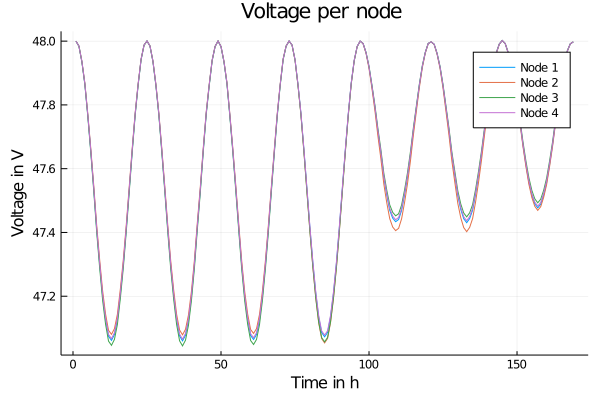
\includegraphics[scale=0.45]{pictures/plots/DC_prosumer_no_ILC_voltage_per_node.png}
	\caption{Voltage $v_{gn,j}(t)$ per node $j=1,2,3,4$ with no higher-layer control for 7 days in hours}
	\label{fig:voltage_no_ILC}
\end{figure}
\begin{figure}[h]
	\centering
	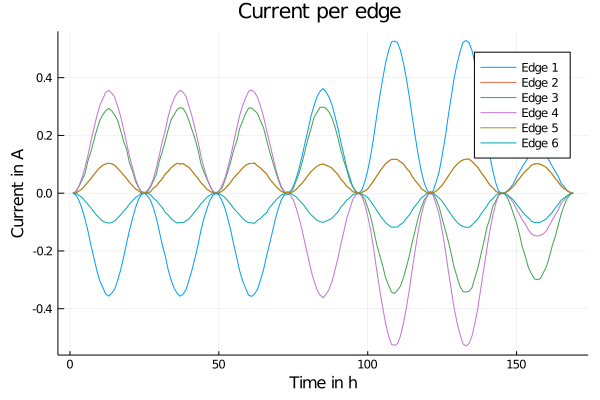
\includegraphics[scale=0.45]{pictures/plots/DC_prosumer_no_ILC_current_per_edge.png}
	\caption{Current per edge with no higher-layer control for 7 days in hours}
	\label{fig:current_no_ILC}
\end{figure}
\begin{figure}[h]
	\centering
	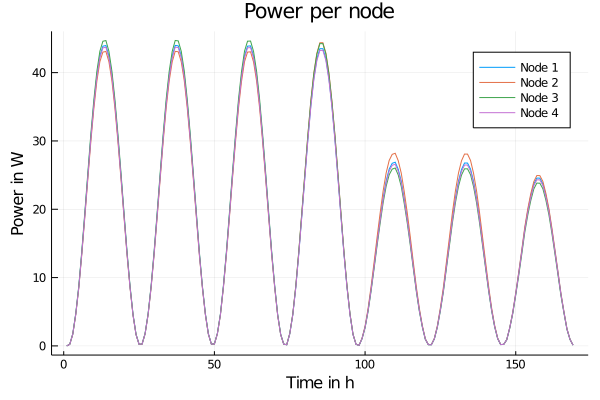
\includegraphics[scale=0.45]{pictures/plots/DC_prosumer_no_ILC_power_per_node.png}
	\caption{Low-level control energy with no higher-layer control for 7 days in hours}
	\label{fig:power_no_ILC}
\end{figure}
\section{Model validation and results of the network with higher-layer control and periodic load profiles}
\label{sec:valid_ILC}
For this section, we now consider the complete derived model of the prosumer-based direct current fully connected microgrid with the iterative learning control and without additional communication. The values of the parameters can be taken from Table \ref{tab:parameters}. 
\\In order to validate the proposed hierarchical controller and to discuss the behavior of it, the two control parameters, the learning parameter of the ILC $\kappa$ and the droop coefficient of the lower-layer control $\boldsymbol{K_D}$ will be varied, so that different case distinctions arise. In particular, we will observe the following cases:
\begin{itemize}
	\item \textbf{Case 1:} Validation of the network modeling with $K_{D,j} = 1$ and $\kappa = 1$ (\ref{subsec:case1})
	\item \textbf{Case 2:} Variation of $\boldsymbol{K_D}$, $\kappa = 1$ (\ref{subsec:case2})
	\item \textbf{Case 3:} Variation of $\kappa$, $K_{D,j} = 1$ (\ref{subsec:case3})
	\item \textbf{Error dynamics for different learning gains}
\end{itemize}
\subsection{Case 1: Validation of the network modeling with $\boldsymbol{K_{D,j} = 1}$ and $\boldsymbol{\kappa = 1}$}
\label{subsec:case1}
Case 1 serves the purpose to validate the overall nonlinear system model (\ref{eq:system}), (\ref{eq:ll_energy}) (\ref{eq:control_ilc}). The main results of case 1 are presented in the following.
\subsubsection*{Description}
Figure \ref{fig:energy_bilance} shows the injected power at the grid nodes. Recall that this is not the low-level control energy. Furthermore, it is the power that is calculated by the product of the voltages $v_{gn,t}(t)$ and the injected currents $i_{gn,t}(t)$ at the grid nodes. 
\\Figure \ref{fig:k1_K1} shows the sum over all nodes of the demand $P_j^d$ (transparent blue), the hourly integrated low-level control energy $y_j^{c,h}$ (red line) and the input from the ILC $u_j^{ILC}$ (black line) for a learning scenario with daily step changes of the peak demand. The peak demand is stepping after four days and again after three or four more days  and is different at each node (Figure \ref{fig:k1_K1}, bottom).As soon as the peak demand steps the low-layer control energy increases on the same day and decreases again on the next day. E.g. a peak of the energy of approx. $\SI{50}{\watt}$ appears on day 5. 

\subsubsection*{Interpretation}
Regarding the injected power of Figure \ref{fig:energy_bilance}, for every hour of the 7 days, the node energies are balanced and power sharing is achieved. This means that if at least one node produces an specific amount of energy, then the remaining node(s) consume this amount, the sum of all injected powers at every grid node is zero. 

Regarding the two-layer control (Figure \ref{fig:k1_K1}) it can be observed that the local ILC learns the local demand. It also steps after four days with a one-day delay (since on Day 1 the ILC does not have learned anything yet). By observing the low-level control energy it can also be determined, that power sharing in the network is achieved through the low-layer control input $u_j^{LI}$ from the first day. The sum of the lower-layer control energy $y^{c,h,s} = \sum_{j}y^{c,h}_j$ is distributed on all 4 nodes proportionally for every $K_{D,j} \in \mathbb{R}_{>0}$ (homogenous scenario).
The following relationship (for every amount of prosumer-nodes) arises:
\begin{align}
N \cdot K_{D,j} \cdot y^{c,h}_j &= y^{c,h,s}, N \in \mathcal{N} \subseteq \mathbb{N}, j={1,2,...,N}, K_{D,j} \in \mathbb{R}_{>0} \label{eq:sum_energy_hom} \\
4 \cdot y^{c,h}_j &= y^{c,h,s} ,N=4, K_{D,j}=1, j=1,2,3,4 \nonumber
\end{align}
Furthermore, the ILC learns based on the synchronized state for the whole network reducing successfully the lower-layer control energy at all nodes. The results of the summed quantities show that, after each demand peak step the ILC learns to compensate the new demand and thereby decreases the low-level control energy to less than $10\%$ of its original value within two days.
\\The fast increase of low-level control energy during the fifth day occurs, since the ILC has not learned yet the new peak demand and therefore reacts by not being able to keep the low-level energy small.
\\Case 1 serves as the "\textit{default}" case for the purpose of validating the network modeling. However, both the low-level and higher-layer controller must be tested in further cases to clarify the conclusions. E.g. in the next case the influence of the control parameter $K_{D,j}$ will be analyzed to confirm the proposed control objectives of power sharing and bounded voltage (\ref{subsec:conobj}).
\begin{figure}[h]
	\centering
	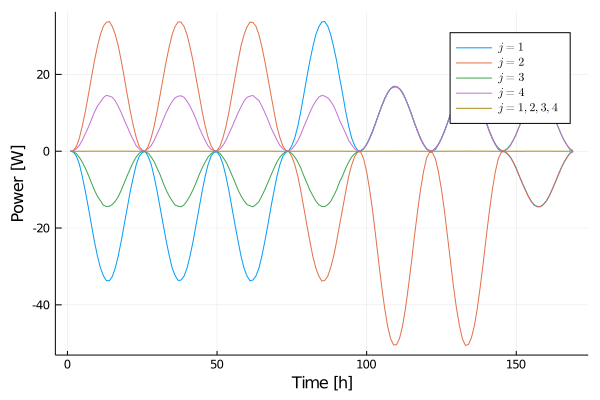
\includegraphics[scale=0.6]{pictures/plots/manual_calc_variation_kappa/kappa_1/K_1/energy_bilance.png}
	\caption{Injected power at every node $j=1,2,3,4$ and the sum (yellow line)}
	\label{fig:energy_bilance}
\end{figure}  
\begin{figure}[h]
	\centering
	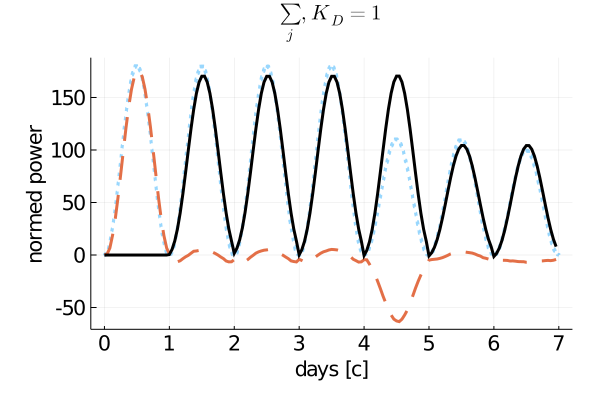
\includegraphics[scale=0.55]{pictures/plots/manual_calc_variation_kappa/kappa_1/K_1/DC_prosumer_demand_seconds_sum_hetero.png}
	
	\bigbreak
	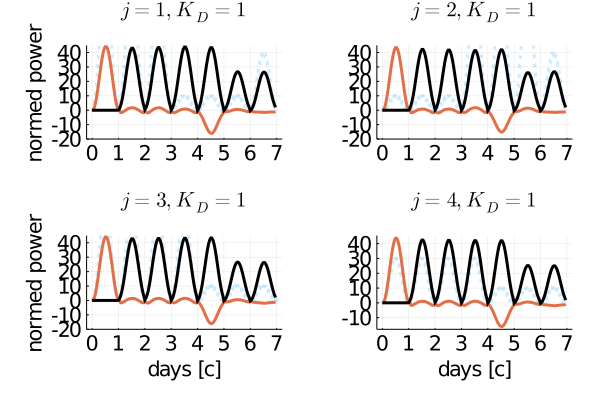
\includegraphics[scale=0.55]{pictures/plots/manual_calc_variation_kappa/kappa_1/K_1/DC_prosumer_demand_seconds_nodes_hetero.png}
	
	
	
	\caption{Top: sum for all nodes $j = 1,2,3,4$, $\kappa = \SI{1}{\hour ^{-1}}$ and $K_{D,j} = \SI{1}{\ohm ^{-1}}$; transparent blue: $\sum_{j} P_j^d$, dashed red: $\sum_{j} y_j^{c,h}$, solid black: $\sum_{j}u_j^{ILC}$; Bottom: seperately for nodes $j = 1,2,3,4$, $\kappa = \SI{1}{\hour ^{-1}}$, $K_{D,j} = \SI{1}{\ohm ^{-1}}$; transparent blue: $P_j^d$, solid red: $y_j^{c,h}$, solid black: $u_j^{ILC}$}
	\label{fig:k1_K1}
\end{figure}

\subsection{Case 2: Variation of  $\boldsymbol{K_D}$ and $\boldsymbol{\kappa = 1}$}
\label{subsec:case2}
Case 2 serves the purpose of analyzing the learning behavior of the hierarchical control for different droop coefficients $K_{D,j}, j=1,2,3,4$ and the influence of this coefficient on the power sharing. For this, K will be set to a vector of different values in order to examine how the variation of droop coefficients affects (quantitatively) the low-level energy. 
\subsubsection*{Description}
Note that the coefficient determines the voltage drop at the output, in our case the difference $V_{ref,j} - v_{gn,j}(t), j=1,2,3,4$.Two different \textit{heterogeneous} scenario have been selected for this case, where different droop coefficients are applied for every node. \textit{Homogeneous} scenarios include the same coefficients on every node. The following droop coefficients $\boldsymbol{K_D} = (K_{D,1},K_{D,2},K_{D,3},K_{D,4})^T$ were used:
\begin{align*}
\boldsymbol{K_{D,a}} = \left(\begin{array}{c} 0.1 \\ 1 \\2\\5 \end{array}\right)\si{\ohm^{-1}} , \boldsymbol{K_{D,b}} = \left(\begin{array}{c} 1 \\ 1 \\0.1\\1 \end{array}\right)\si{\ohm^{-1}} 
\end{align*}
Four different values have been assigned for every node in $\boldsymbol{K_{D,a}}$ and one different value in $\boldsymbol{K_{D,b}}$.
Figures \ref{fig:k1_KDa} and \ref{fig:k1_KDb} show the demand $P_j^d$ (transparent blue), the hourly integrated low-level control energy $y_j^{c,h}$ (red line) and the input from the ILC $u_j^{ILC}$ (black line) and the sums $\sum_{j}P_j^d$, $\sum_{j}y_j^{c,h}$ and $\sum_{j}u_j^{ILC}$ for learning scenarios with daily step changes of the peak demand for the droop coefficient $\boldsymbol{K_{D,a}}$ and $\boldsymbol{K_{D,b}}$, respectively, $j=1,2,3,4$. 

\paragraph{$\boldsymbol{K_{D,a}}$:} 
Changing the droop coefficient for every node obviously changes also the value of the daily low-level control energy. E.g. in node 1, the droop coefficient $K_{D,a,1} = \SI{0.1}{\ohm^{-1}}$ was applied. Since this parameter is also an immediate part of $u^{LI}$ (Eq. \ref{eq:ll_energy}) the hourly integrated energy is reduced by almost $\frac{1}{10}$ compared to the energy on node 2 with $K_{D,a,2} = \SI{1}{\ohm^{-1}}$ . However, the energy on node 2 is smaller than the energies in Case 1 ($K_{D,j} = \SI{1}{\hour^{-1}}$). For node 4, the droop coefficient $K_{D,a,4} = \SI{5}{\ohm^{-1}}$ was applied. The integrated energy in this node is almost 5 times bigger compared to node 2. Increased, i.e. decreased lower-layer control energy leads to equivalently increased, i.e. decreased ILC power, which can also be observed in Figure \ref{fig:k1_KDa}. The sum of powers on each node is observed to be equivalent compared to Case 1 ($K_{D,j} = \SI{1}{\hour^{-1}}$). 
\paragraph{$\boldsymbol{K_{D,b}}$:}
In this case, it is observed that that nodes $j=1$, $j=2$ and $j=4$, where the droop coefficient $\SI{1}{\hour^{-1}}$ is applied show the same amount of low-level control energy. The energies are bigger than the Case 1 ($K_{D,j} = \SI{1}{\hour^{-1}}$) energies with the same droop coefficient. For node $j=3$ with $K_{D,b,3} = \SI{0.1}{\hour^{-1}}$ the energy is reduced by almost $\frac{1}{10}$ compared to the other nodes. The sum of powers on each node is equivalent compared to Case 1 ($K_{D,j} = \SI{1}{\hour^{-1}}$). 
\begin{figure}[h]
	\centering
	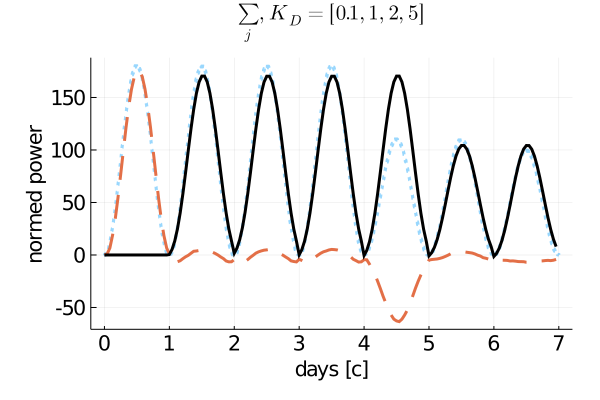
\includegraphics[scale=0.55]{pictures/plots/manual_calc_variation_kappa/kappa_1/K_variance/KDa/DC_prosumer_demand_seconds_sum_hetero.png}

	\bigbreak
	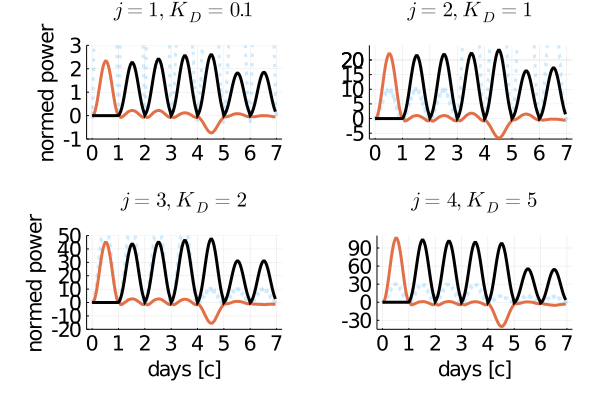
\includegraphics[scale=0.55]{pictures/plots/manual_calc_variation_kappa/kappa_1/K_variance/KDa/DC_prosumer_demand_seconds_nodes_hetero.png}



	\caption{Top: sum for all nodes $j = 1,2,3,4$, $\kappa = \SI{1}{\hour ^{-1}}$ and $\boldsymbol{K_{D,a}} = (0.1,1,2,5)^T\si{\ohm ^{-1}}$; transparent blue: $\sum_{j} P_j^d$, dashed red: $\sum_{j} y_j^{c,h}$, solid black: $\sum_{j}u_j^{ILC}$; Bottom: seperately for nodes $j = 1,2,3,4$, $\kappa = \SI{1}{\hour ^{-1}}$, $\boldsymbol{K_{D,a}} = (0.1,1,2,5)^T\si{\ohm ^{-1}}$; transparent blue: $P_j^d$, solid red: $y_j^{c,h}$, solid black: $u_j^{ILC}$}
	\label{fig:k1_KDa}
\end{figure}

\subsubsection*{Interpretation}
The higher the droop coefficient is, the smaller is the difference between the two voltages. A higher droop coefficient also means a faster reaction of the currents, resulting increasing currents. The low-level control energy per node increases for increasing $K_{D,j}$ and decreases for decreasing $K_{D,j}$, respectively.
\\The sum of the low-layer control energy at every node of the nonlinear model $y^{c,h,s} = \sum_{j}y^{c,h}_j$ with the parameters of Table \ref{tab:parameters} is for every $K_{D,j}\in \mathbb{R}_{>0}$ equal. Changing the droop coefficient in a heterogenous scenario will only change the distribution of the integrated energies on every node and therefore the value of integrated energies per node.
A higher droop coefficient at a node will increase the lower-layer control energy there and reduce it on the rest of the nodes. Likewise the reduction of the droop coefficient at a node will increase the energy of the other nodes. The sum of powers at every node is distributed on all nodes proportionally, depending on the coefficient. 
For every heterogenous scenario the following relationship arises:
\begin{align}
\sum_{j}^{N} K_{D,j} \cdot y^{c,h}_j = y^{c,h,s},N \in \mathcal{N} \subseteq \mathbb{N},j&={1,2,...,N},K_{D,j} \in \mathbb{R}_{>0} \label{eq:sum_energy_het} \\
0.1 \cdot y^{c,h}_1 + y^{c,h}_2 + 2 \cdot y^{c,h}_3 + 5 \cdot y^{c,h}_4 &= y^{c,h,s}, j=1,2,3,4, N=4, \boldsymbol{K_{D}} = \boldsymbol{K_{D,a}} \nonumber  \\
y^{y,h}_1 + y^{c,h}_2 + 0.1 \cdot y^{c,h}_3 + y^{c,h}_4 &= y^{c,h,s},j=1,2,3,4, N=4, \boldsymbol{K_{D}} = \boldsymbol{K_{D,b}} \nonumber
\end{align}
Fair power sharing is achieved for all prosumers. This is necessary in order to assure the same rights for each user regardless of the position in the microgrid. In other words, when a prosumer of the grid feeds a greater amount of power into the grid, the other prosumer will feed a equivalently smaller amount of power intro the grid, to keep the total energy balance of the microgrid.
\\As also in Case 1 ($K_{D,j} = \SI{1}{\hour^{-1}}$), the peak demand steps after four days and again after 3 days and is different at each node (Figures \ref{fig:k1_KDa} and \ref{fig:k1_KDb},bottom). The local ILC learns to compensate the new local demand after each demand peak step, stepping with the same frequency as the local demand and the low-level control energy decreases also after the day after the ILC has learned the new periodic demand. 
\\The next case varies the learning parameter $\kappa$ for a constant droop coefficient $K_{D,j}= \SI{1}{\ohm^{-1}}$ to analyze the learning behavior of the iterative learning controller.
\begin{figure}[h]
	\centering
	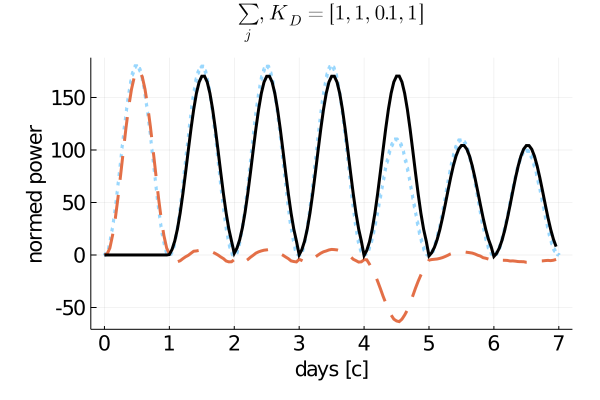
\includegraphics[scale=0.55]{pictures/plots/manual_calc_variation_kappa/kappa_1/K_variance/KDb/DC_prosumer_demand_seconds_sum_hetero.png}
	
	\bigbreak
	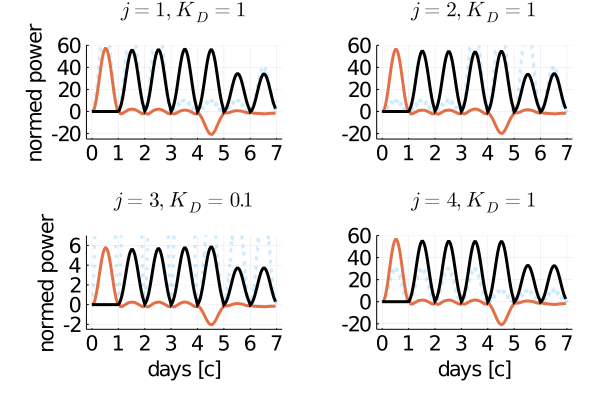
\includegraphics[scale=0.55]{pictures/plots/manual_calc_variation_kappa/kappa_1/K_variance/KDb/DC_prosumer_demand_seconds_nodes_hetero.png}
	
	
	
	\caption{Top: sum for all nodes $j = 1,2,3,4$, $\kappa = \SI{1}{\hour ^{-1}}$ and $\boldsymbol{K_{D,b}} = (1,1,0.1,1)^T\si{\ohm ^{-1}}$; transparent blue: $\sum_{j} P_j^d$, dashed red: $\sum_{j} y_j^{c,h}$, solid black: $\sum_{j}u_j^{ILC}$; Bottom: seperately for nodes $j = 1,2,3,4$, $\kappa = \SI{1}{\hour ^{-1}}$, $\boldsymbol{K_{D,b}} = (1,1,0.1,1)^T\si{\ohm ^{-1}}$; transparent blue: $P_j^d$, solid red: $y_j^{c,h}$, solid black: $u_j^{ILC}$}
	\label{fig:k1_KDb}
\end{figure}
\subsection{Case 3: Variation of  $\boldsymbol{\kappa}$ and $\boldsymbol{K_{D,j}= \SI{1}{\ohm^{-1}}}$}
\label{subsec:case3}
\label{subsec:K_1_kappa_var}
Case 3 serves the purpose of analyzing the learning behavior of the hierarchical control for different learning parameter $\kappa \in ]0,2[ \si{hour^{-1}}$. 
\\Figure \ref{fig:kvar_KD1} presents the sum over all nodes of the demand $\sum_{j}P^d_j$, the low-level control energy $\sum_{j}y^{c,h}_j$ and the input from the ILC $\sum_{j} u^{ILC}_j$ for a learning scenario with artificial step changes of the peak demand for a variety of different learning parameter $\kappa$. 
\subsubsection*{Observations}
\paragraph{$\boldsymbol{\kappa \in ]0,1[\si{\hour^{-1}}}$:}
For $\kappa \in ]0,1[\si{\hour^{-1}}$ the ILC power regulates slowly during the second days and learns the first peak of demand. During the fifth day, for $\kappa = \SI{0.25}{\hour^{-1}}$ the ILC has reached almost $70\%$ of the demand and in the next days it regulates to the next amplitude. For $\kappa = \SI{0.5}{\hour^{-1}}$ and $\kappa = \SI{0.75}{\hour^{-1}}$ the learning improves, while the ILC power approaches during the fifth day the peak demand. However, the response for $\kappa \in ]0,1[\si{\hour^{-1}}$ is slower than for $\kappa = \SI{1}{\hour^{-1}}$, where the ILC has reached the amount of the demand power during the second day. 
\\In addition the low-level control energy decreases for $\kappa \in ]0,1[\si{\hour^{-1}}$, with a bigger $\kappa$ having a faster decrease as result. E.g. the sum of low-level control energy over all nodes decreases faster for $\kappa = \SI{0.75}{\hour^{-1}}$ than for $\kappa = \SI{0.5}{\hour^{-1}}$. The negative peak of the energy that is observed for $\kappa = \SI{1}{\hour^{-1}}$ in Figure \ref{fig:k1_K1} grows with an increasing $\kappa$.
\paragraph{$\boldsymbol{\kappa \in ]1,2[\si{\hour^{-1}}}$:}
For $\kappa$ in $]1,2[\si{\hour^{-1}}$  the ILC shows a quick regulation during the second day and learns the first peak of demand. The more $\kappa$ increases the bigger the amount of the power in the second day gets and the more the learning behavior of the ILC downgrades, as it shows a variety of different amplitudes. E.g. in Figure \ref{fig:kvar_KD1} for $\kappa = \SI{1.5}{\hour^{-1}}$  the demand amplitude is $180$ during the four first days and the ILC shows an amplitude of $250$ in the second and an amplitude of approx. $130$ in the third day  For $\kappa = \SI{1}{\hour^{-1}}$  the ILC learn the demand by adapting the amplitudes of $180$ immediately after the first day. 
\\The lower-layer control energy over all nodes decreases in $\mathbb{R}_{>0}$ and increases in $\mathbb{R}_{<0}$ after the first day for all $\kappa = ]1,2[\si{\hour^{-1}}$ , while the negative peak during the fifth day ($\kappa = \SI{1}{\hour^{-1}}$ ) decreases.

\subsubsection*{Interpretation}
If one compares the single representations from Figure \ref{fig:kvar_KD1} with each other, as well as with the representation in Figure \ref{fig:k1_K1}, one quickly notices that in the interval $\kappa \in ]0,1[\si{\hour^{-1}}$ the learning behavior of the iterative learning controller improves for increasing $\kappa$ and deteriorates for increasing $\kappa$ in $]1,2[\si{\hour^{-1}}$. For $\kappa = \SI{1}{\hour^{-1}}$ the learning scenario is the most efficient. The controller reacts sensitive to the change of the demand amplitudes, so that the integrated energy increases again, until the controller has learned the demand. In the next Section it will be studied how the error convergence in the iteration domain depends on the choice of the scalar learning parameter.

\subsection{Error dynamics for different learning gains}
\label{subsec:error_dyn}
We study how the error convergence in the iteration domain depends on the choice of the scalar learning parameter $\kappa$. Again, the nonlinear model with the two-layer control is used with modified demand pattern \cite{paperilc}. The periodic peak demand is between $0.6$ and $\SI{0.9}{\watt / \watt}$ at the different nodes and the fluctuating component varies randomly from day to day within $[-0.7,0.7]$$\si{\watt / \watt}$. The smaller amplitudes of the demand in this case ensure that the increased low-level energy on day 5 from the upper sections  are again minimised. 
\\Different values of $\kappa = [0,2]\si{\hour^{-1}}$  are considered. For each value, the error norm, i.e. a measure of the overall low-level control energy is calculated for each of the 20 first days \cite{paperilc}. Figure \ref{fig:error_norm} shows the results of the study. For $\kappa \in [0,1]$ the error norm converges faster for increasing $\kappa$. The error norm is constant for $\SI{0}{\hour^{-1}}$ (no learning) over the cycles. For $\kappa \in [1,2]$ the error norm converges slower for increasing $\kappa$, i.e the error norm is not converging for $\kappa = \SI{2}{\hour^{-1}}$. The convergence of the error norm is therefore fastest for $\kappa = \SI{1}{\hour^{-1}}$. This observation confirms the statement from Case 3, that for $\kappa = \SI{1}{\hour^{-1}}$ the learning scenario is the optimal. 
\begin{figure}[!tbp]
	\centering
	\begin{minipage}[b]{0.475\textwidth}
		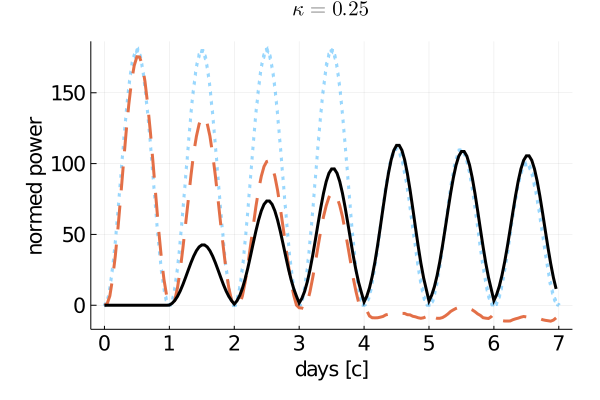
\includegraphics[width=\textwidth]{pictures/plots/manual_calc_variation_kappa/kappa_025_energies_sum.png}
		
	\end{minipage}
	\hfill
	\begin{minipage}[b]{0.475\textwidth}
		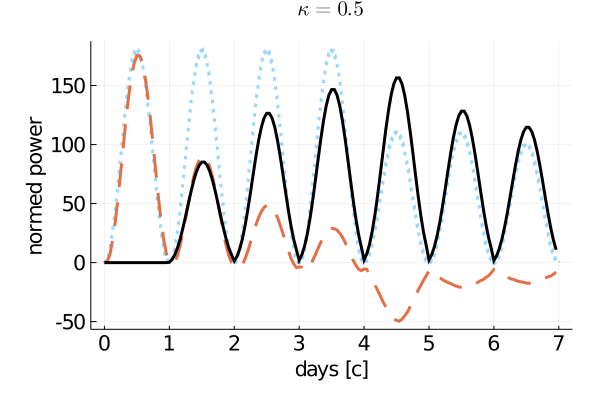
\includegraphics[width=\textwidth]{pictures/plots/manual_calc_variation_kappa/kappa_05_energies_sum.png}
		
	\end{minipage}
\end{figure}
\begin{figure}[!tbp]
	\centering
	\begin{minipage}[b]{0.475\textwidth}
		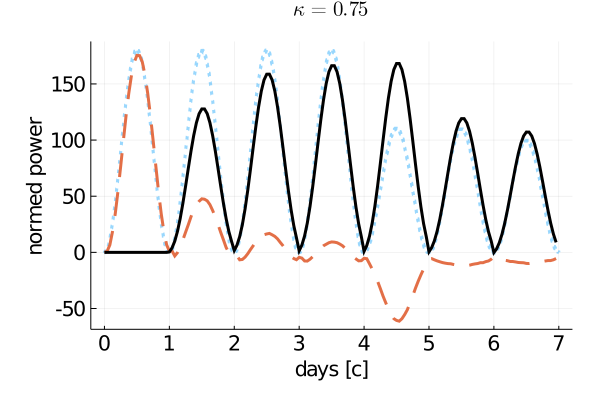
\includegraphics[width=\textwidth]{pictures/plots/manual_calc_variation_kappa/kappa_075_energies_sum.png}
		
	\end{minipage}
	\hfill
	\begin{minipage}[b]{0.475\textwidth}
		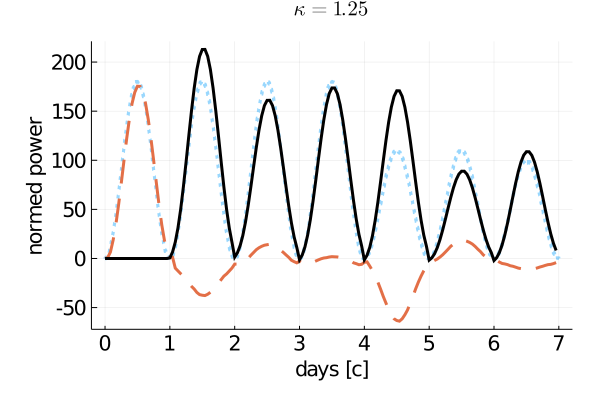
\includegraphics[width=\textwidth]{pictures/plots/manual_calc_variation_kappa/kappa_125_energies_sum.png}
		
	\end{minipage}
\end{figure}
\begin{figure}[!tbp]
	\centering
	\begin{minipage}[b]{0.475\textwidth}
		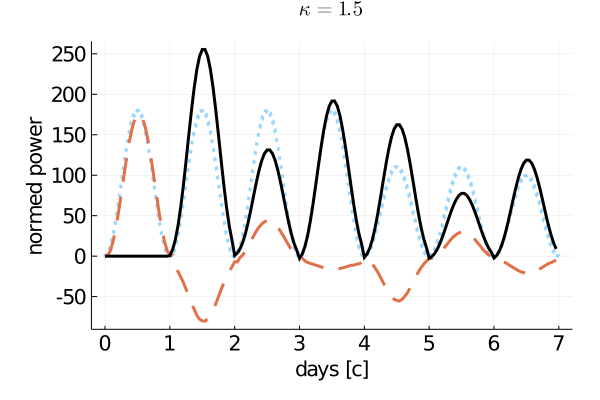
\includegraphics[width=\textwidth]{pictures/plots/manual_calc_variation_kappa/kappa_15_energies_sum.png}
		
	\end{minipage}
	\hfill
	\begin{minipage}[b]{0.475\textwidth}
		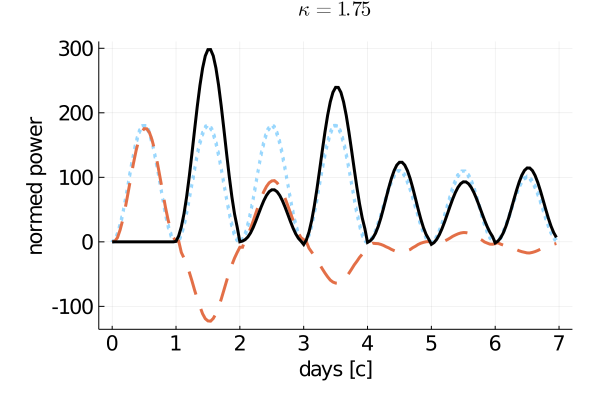
\includegraphics[width=\textwidth]{pictures/plots/manual_calc_variation_kappa/kappa_175_energies_sum.png}
		
	\end{minipage}
	\caption{sum for all nodes $j = 1,2,3,4$ with $K_{D,j} = 1\si{\ohm ^{-1}}$; Top left: $\kappa = \SI{0.25}{\hour ^{-1}}$; Top right: $\kappa = \SI{0.5}{\hour ^{-1}}$; Center left: $\kappa = \SI{0.75}{\hour ^{-1}}$; Center right: $\kappa = \SI{1.25}{\hour ^{-1}}$; Bottom left: $\kappa = \SI{1.5}{\hour ^{-1}}$; Bottom right: $\kappa = \SI{1.75}{\hour ^{-1}}$; transparent blue: $\sum_{j} P_j^d$, dashed red: $\sum_{j} y_j^{c,h}$, solid black: $\sum_{j}u_j^{ILC}$;}
	\label{fig:kvar_KD1}
\end{figure}
\begin{figure}[h]
	\centering
	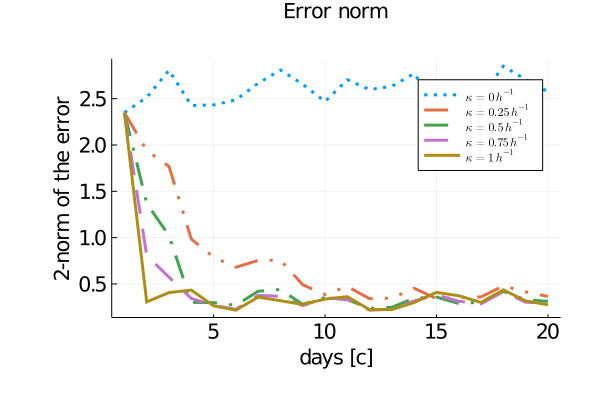
\includegraphics[scale=0.6]{pictures/plots/manual_calc_variation_kappa/variation_kappa_leq_1_hetero.png}
	\bigbreak
	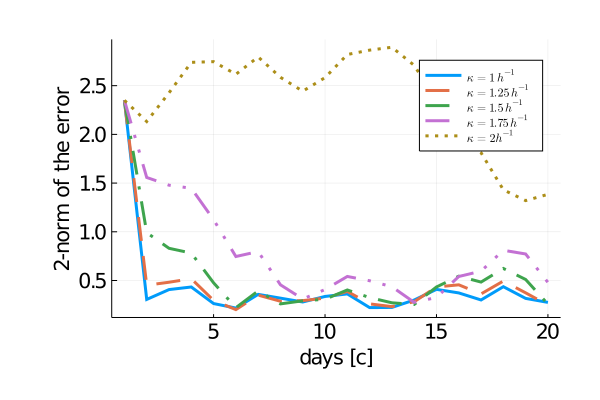
\includegraphics[scale=0.6]{pictures/plots/manual_calc_variation_kappa/variation_kappa_geq_1_hetero.png}
	\caption{Error norm ($||\boldsymbol{e}^c||_2$) over the days for different learning gains with the nonlinear simulation}
	\label{fig:error_norm}
\end{figure} 

\section{Discussion}
Taking all results from Sections \ref{sec:valid_no_ILC} and \ref{sec:valid_ILC} for the prosumer-based direct current microgrid with iterative learning control, it can be said that:
\begin{enumerate}
	\item The suggested prosumer-based direct current microgrid framework (Eq. \ref{eq:system}) with lower-layer control (Eq. \ref{eq:ll_energy}) achieves voltage droop and power sharing with the corresponding droop coefficient $\boldsymbol{K_{D}}$. Depending on the individual purposes, e.g. if a specific prosumer should produce/consume a bigger amount of power, the coefficient, as well as the compound plant parameters can be varied. For an equal distribution of power inbetween the nodes, choosing for the droop coefficient $K_{D,j} = \SI{1}{\ohm^{-1}}$ will complete this purpose.
	\item The suggested iterative learning controller (Eq. \ref{eq:control_ilc}) not only learned the local demand and contributed with the low-level controller by ensuring the power sharing. Instead, it saved the low-level control energy, showing some sensitivity, whenever the peak demand changed.
	\item The low-level control energy was decreased for almost every learning parameter $\kappa$. By calculating the error convergence for the low-level control energy, it was showed that the optimal learning behavior is achieved at $\kappa = \SI{1}{\hour^{-1}}$. 
\end{enumerate}


\chapter{Conclusions}
\label{sec:conclusions}
The thesis and results presented in the previous sections will be summarized in Section \ref{sec:summary}. Further, a number of recommendations for future work will be provided in Section \ref{sec:future}.

\section{Summary of the thesis}
\label{sec:summary}
We propose a framework for a hierarchical control in a prosumer-based direct current microgrid with suitable parameters.
The prosumer-based network modeling is derived from the already existing producer-consumer scheme and the Kirchhoff Laws (Section \ref{subsec:prosumer}). For the low-level control, a controller with the main focus on power sharing and voltage droop was applied (Section \ref{subsec:conobj}). By choosing the appropriate control coefficient, power sharing was achieved, as seen in the simulation in Section \ref{sec:valid_no_ILC} and \ref{sec:valid_ILC}. 
For the higher-layer control the predefined iterative learning controller was applied, a controller that learns the periodic demand pattern in order to save as much low-level control energy (Section \ref{sec:ilc_design}) and by choosing the appropriate learning parameter, the learning scenario can achieved different velocities, while power sharing and voltage droop is guaranteed.

\section{Future Work}
\label{sec:future}
In the future, the analysis of the iterative learning control in a prosumer-based direct current microgrid by implementing a lifted system for asymptotic stability and monotonic convergence should be developed. Furthermore,  viewing the learning scenario with real demand data and comparing it to the already existing prosumer-based alternating current microgrid from \cite{paperilc} are tasks that could be done. 



\bibliography{literature}
\bibliographystyle{IEEEtran}
\nocite{paperilc}
\nocite{dg_wiki}
\nocite{epa_dg}
\nocite{Hatzi}
\nocite{concept}
\nocite{microgrid_concept}
\nocite{versus}
\nocite{lineloss}
\nocite{portm}
\nocite{prosumage}
\nocite{prosume}
\nocite{un_graph}
\nocite{graph_theory}
\nocite{lia_master}
\nocite{lia_stability}
\nocite{xiaohan_master}
\nocite{cs_princi}
\nocite{cs_princi_wiki}
\nocite{oploop}
\nocite{hier_control}
\nocite{controldc}
\nocite{controldc_energy_man}
\nocite{vl_ilc}
\nocite{moore_ilc}
\nocite{reduced_dc}
\nocite{voltage_droop}
\nocite{mikieus}

\chapter*{Appendix}
\label{appendix}
This chapter contains the sample code of the simulation framework utilized in this thesis in Section A and the sample code for the error norm calculation in Section B. 
\section*{A Simulation code}

\begin{lstlisting}
begin
using JLD2, FileIO, GraphIO, CSV, DataFrames
using ForwardDiff
using Distributed
using LightGraphs # create network topologies
using LinearAlgebra
using DifferentialEquations
using GraphPlot
using Random
using NetworkDynamics
using Plots
using Parameters
using ToeplitzMatrices
using DSP
using LaTeXStrings
using Distributions
using StatsBase
using Roots
using Interpolations
Random.seed!(42)
end

begin
dir = @__DIR__
N = 4 #Number of nodes
N_half = Int(N/2)
num_days = 7
l_day = 3600*24 # DemCurve.l_day
l_hour = 3600 # DemCurve.l_hour
l_minute = 60
end

struct demand_amp_var
demand
end

function (dav::demand_amp_var)(t)
index = Int(floor(t / (24*3600)))
dav.demand[index + 1,:]
end

begin
graph = random_regular_graph(iseven(3N) ? N : (N-1), 3)
end

@with_kw mutable struct LeakyIntegratorPars
K
R
L_inv
C_inv
v_ref
n_prod
n_cons
end

@with_kw mutable struct ILCPars
kappa
mismatch_yesterday
daily_background_power
current_background_power
ilc_nodes
ilc_covers
Q
end

@with_kw mutable struct incidences
inc_i
inc_v
end

@with_kw mutable struct UlMoparss
N::Int
ll::LeakyIntegratorPars
hl::ILCPars
inc::incidences
periodic_infeed
periodic_demand
fluctuating_infeed
residual_demand
incidence

function UlMoparss(N::Int,
ll::LeakyIntegratorPars,
hl:: ILCPars,
inc::incidences,
periodic_infeed,
periodic_demand,
fluctuating_infeed,
residual_demand)
new(N, ll,
hl,
inc,
periodic_infeed,
periodic_demand,
fluctuating_infeed,
residual_demand,
incidence_matrix(graph,oriented=true))
end
end

function set_parameters(N, kappa, Q)
low_layer_control = LeakyIntegratorPars(K = 1., R = 0.0532, L_inv = 1/0.237e-4, C_inv = 1/0.01,  v_ref = 48. ,  n_prod = num_prod, n_cons = N.-num_prod)
control_incidences = incidences(inc_i = zeros(N), inc_v = zeros(Int(1.5*N)))
higher_layer_control = ILCPars(kappa = kappa, mismatch_yesterday=zeros(24,N), daily_background_power=zeros(24,N), current_background_power=zeros(N), ilc_nodes=1:N, ilc_covers = [], Q = Q)
periodic_infeed = t -> zeros(N)
peak_demand = rand(N)
periodic_demand = t -> zeros(N)
fluctuating_infeed = t -> zeros(N)
residual_demand = t -> zeros(N)

return UlMoparss(N,low_layer_control,
higher_layer_control,
control_incidences,
periodic_infeed,
periodic_demand,
fluctuating_infeed,
residual_demand)
end

begin
current_filter = 1:Int(1.5N)
voltage_filter = Int(1.5N)+1:Int(2.5N)
energy_filter = Int(2.5N)+1:Int(3.5N)#3N+1:4N
end

function prosumerToymodel!(du, u, p, t)
n_lines = Int(1.5*p.N)

#state variables
i = u[1:n_lines]
v = u[(n_lines+1):Int(2.5*p.N)]
di = @view du[1:n_lines]
dv = @view du[(n_lines+1):Int(2.5*p.N)]
control_power_integrator = @view du[Int(2.5*p.N)+1:Int(3.5*p.N)]

periodic_power =  p.periodic_demand(t) .+ p.periodic_infeed(t) #determine the update cycle of the hlc
fluctuating_power =   p.residual_demand(t) .+ p.fluctuating_infeed(t) # here we can add fluctuating infeed as well
Pd = periodic_power + fluctuating_power # Demand

i_ILC =  p.hl.current_background_power./v # power ILC in form of a current

p.inc.inc_v = p.incidence' * v
p.inc.inc_i = p.incidence * i
i_gen = p.ll.K .* (p.ll.v_ref .- v) # generated current
i_load = Pd./(v.+1) # load current

#differential equations
@. di = p.ll.L_inv .*(-(p.ll.R.*i) .+ p.inc.inc_v)
@. dv = p.ll.C_inv.*(i_ILC.+i_gen.- p.inc.inc_i .- i_load)
@. control_power_integrator = i_gen.* v 	#power LI

return nothing
end

@doc """
HourlyUpdate()
Store the integrated control power in memory.
See also [`(hu::HourlyUpdate)`](@ref).
"""
struct HourlyUpdate
integrated_control_power_history
HourlyUpdate() = new([])
end

@doc """
HourlyUpdate(integrator)
PeriodicCallback function acting on the `integrator` that is called every simulation hour (t = 1,2,3...).
"""
function (hu::HourlyUpdate)(integrator)
hour = mod(round(Int, integrator.t/3600.), 24) + 1
last_hour = mod(hour-2, 24) + 1
power_idx = Int(2.5*integrator.p.N)+1:Int(3.5*integrator.p.N) # power index

#power calculation y^c
integrator.p.hl.mismatch_yesterday[last_hour,:] .= 1/3600 .* integrator.u[power_idx]
integrator.u[power_idx] .= 0.

integrator.p.hl.current_background_power .= integrator.p.hl.daily_background_power[hour, :]

nothing
end

function DailyUpdate_X(integrator)
#ilc
integrator.p.hl.daily_background_power =  integrator.p.hl.Q * (integrator.p.hl.daily_background_power + integrator.p.hl.kappa .* integrator.p.hl.mismatch_yesterday)
nothing
end

demand_amp1 = demand_amp_var(repeat([80 80 80 10 10 10 40 40 40 40 40], outer=Int(N/4))') # random positive amp over days by 10%
demand_amp2 = demand_amp_var(repeat([10 10 10 80 80 80 40 40 40 40 40], outer=Int(N/4))') # random positive amp over days by 10%
demand_amp3 = demand_amp_var(repeat([60 60 60 60 10 10 10 40 40 40 40], outer=Int(N/4))') # random positive amp over days by 10%
demand_amp4 = demand_amp_var(repeat([30 30 30 30 10 10 10 80 80 80 80], outer=Int(N/4))') # random positive amp over days by 10%
demand_amp = t->vcat(demand_amp1(t), demand_amp2(t), demand_amp3(t), demand_amp4(t))


periodic_demand =  t-> demand_amp(t) .* sin(t*pi/(24*3600))^2
samples = 24*4
inter = interpolate([.2 * randn(N) for i in 1:(num_days * samples + 1)], BSpline(Linear()))
residual_demand = t -> inter(1. + t / (24*3600) * samples)

##################  set higher_layer_control ##################

kappa = 1.
vc1 = 1:N # ilc_nodes (here: without communication)
cover1 = Dict([v => [] for v in vc1])# ilc_cover
u = [zeros(1000,1);1;zeros(1000,1)];
fc = 1/6;
a = digitalfilter(Lowpass(fc),Butterworth(2));
Q1 = filtfilt(a,u);# Markov Parameter
Q = Toeplitz(Q1[1001:1001+24-1],Q1[1001:1001+24-1]);

################### set parameters ############################
begin
param = set_parameters(N, kappa, Q)
param.periodic_demand = periodic_demand
param.residual_demand = residual_demand
param.hl.daily_background_power .= 0
param.hl.current_background_power .= 0
param.hl.mismatch_yesterday .= 0.
end
####################### solving ###############################
begin
fp = [0. 0. 0. 0. 0. 0. 48. 48. 48. 48. 0. 0. 0. 0.] #initial condition
factor = 0.
ic = factor .* ones(14)
tspan = (0. , num_days * l_day) # 1 Tag
tspan2 = (0., 10.0)
#tspan3 = (0., 200.)
ode = ODEProblem(prosumerToymodel!, fp, tspan, param,
callback=CallbackSet(PeriodicCallback(HourlyUpdate(), l_hour),
PeriodicCallback(DailyUpdate_X, l_day)))
end
sol = solve(ode, Rodas4())


#################################################################################
######################## ENERGIES ########################################
hourly_energy = zeros(24*num_days+1,N)

for i=1:24*num_days+1
for j = 1:N
hourly_energy[i,j] = sol((i-1)*3600)[energy_filter[j]]./3600 #the hourly integrated low-level control energy
end
end

ILC_power = zeros(num_days+2,24,N)
for j = 1:N
ILC_power[2,:,j] = Q*(zeros(24,1) +  kappa*hourly_energy[1:24,j]) # the ILC power
end
norm_energy_d = zeros(num_days,N)
for j = 1:N
norm_energy_d[1,j] = norm(hourly_energy[1:24,j])
end

for i=2:num_days
for j = 1:N
ILC_power[i+1,:,j] = Q*(ILC_power[i,:,j] +  kappa*hourly_energy[(i-1)*24+1:i*24,j])
norm_energy_d[i,j] = norm(hourly_energy[(i-1)*24+1:i*24,j])
end
end

ILC_power_agg = [norm(mean(ILC_power,dims=3)[d,:]) for d in 1:num_days+2]
ILC_power_hourly_mean = vcat(mean(ILC_power,dims=3)[:,:,1]'...)
ILC_power_hourly_mean_node1 = vcat(ILC_power[:,:,1]'...)
ILC_power_hourly = [norm(reshape(ILC_power,(num_days+2)*24,N)[h,:]) for h in 1:24*(num_days+2)]
ILC_power_hourly_node1 = [norm(reshape(ILC_power,(num_days+2)*24,N)[h,1]) for h in 1:24*(num_days+2)]
dd = t->((-periodic_demand(t) .- residual_demand(t)))
load_amp = [first(maximum(dd(t))) for t in 1:3600*24:3600*24*num_days]

norm_hourly_energy = [norm(hourly_energy[h,:]) for h in 1:24*num_days]

################################## PLOTTING ########################################


node = 1
p1 = plot()
ILC_power_hourly_mean_node = vcat(ILC_power[:,:,node]'...)
plot!(0:num_days*l_day, t -> -dd(t)[node], alpha=0.2, label = latexstring("P^d_$node"),linewidth=3, linestyle=:dot)
plot!(1:3600:24*num_days*3600,hourly_energy[1:num_days*24,node], label=latexstring("y_$node^{c,h}"),linewidth=3) #, linestyle=:dash)
plot!(1:3600:num_days*24*3600,  ILC_power_hourly_mean_node[1:num_days*24], label=latexstring("\$u_$node^{ILC}\$"), xticks = (0:3600*24:num_days*24*3600, string.(0:num_days)), ytickfontsize=14,
xtickfontsize=14,
legendfontsize=10, linewidth=3, yaxis=("normed power",font(14)),legend=false, lc =:black, margin=5Plots.mm)
title!(latexstring("j = $(node), K_D = 1"))
ylims!(-25,60)
savefig("$dir/plots/kappa_1/K_variance/K=[0.1,0.1,1,0.1]/DC_prosumer_demand_seconds_$(node)_hetero.png")


node = 2
p2 = plot()
ILC_power_hourly_mean_node = vcat(ILC_power[:,:,node]'...)
plot!(0:num_days*l_day, t -> -dd(t)[node], alpha=0.2, label = latexstring("P^d_$node"),linewidth=3, linestyle=:dot)
plot!(1:3600:24*num_days*3600,hourly_energy[1:num_days*24,node], label=latexstring("y_$node^{c,h}"),linewidth=3) #, linestyle=:dash)
plot!(1:3600:num_days*24*3600,  ILC_power_hourly_mean_node[1:num_days*24], label=latexstring("\$u_$node^{ILC}\$"), xticks = (0:3600*24:num_days*24*3600, string.(0:num_days)), ytickfontsize=14,
xtickfontsize=14,
legendfontsize=10, linewidth=3,legend=false, lc =:black, margin=5Plots.mm)
#savefig("$dir/plots/kappa_1/DC_prosumer_demand_seconds_node_$(node)_hetero.png")
title!(latexstring("j = $(node), K_D = 1"))
ylims!(-25,60)
savefig("$dir/plots/kappa_1/K=1/DC_prosumer_demand_seconds_$(node)_hetero.png")

node = 3
p3 = plot()
ILC_power_hourly_mean_node = vcat(ILC_power[:,:,node]'...)
plot!(0:num_days*l_day, t -> -dd(t)[node], alpha=0.2, label = latexstring("P^d_$node"),linewidth=3, linestyle=:dot)
plot!(1:3600:24*num_days*3600,hourly_energy[1:num_days*24,node], label=latexstring("y_$node^{c,h}"),linewidth=3) #, linestyle=:dash)
plot!(1:3600:num_days*24*3600,  ILC_power_hourly_mean_node[1:num_days*24], label=latexstring("\$u_$node^{ILC}\$"), xticks = (0:3600*24:num_days*24*3600, string.(0:num_days)), ytickfontsize=14,
xtickfontsize=14,
legendfontsize=10, linewidth=3, xaxis = ("days [c]",font(14)),yaxis=("normed power",font(14)),legend=false, lc =:black, margin=5Plots.mm)
#savefig("$dir/plots/kappa_1/DC_prosumer_demand_seconds_node_$(node)_hetero.png")
title!(latexstring("j = $(node), K_D = 0.1"))
ylims!(-2.5,7)
savefig("$dir/plots/kappa_1/K=1/DC_prosumer_demand_seconds_$(node)_hetero.png")

node = 4
p4 = plot()
ILC_power_hourly_mean_node = vcat(ILC_power[:,:,node]'...)
plot!(0:num_days*l_day, t -> -dd(t)[node], alpha=0.2, label = latexstring("P^d_$node"),linewidth=3, linestyle=:dot)
plot!(1:3600:24*num_days*3600,hourly_energy[1:num_days*24,node], label=latexstring("y_$node^{c,h}"),linewidth=3) #, linestyle=:dash)
plot!(1:3600:num_days*24*3600,  ILC_power_hourly_mean_node[1:num_days*24], label=latexstring("\$u_$node^{ILC}\$"), xticks = (0:3600*24:num_days*24*3600, string.(0:num_days)), ytickfontsize=14,
xtickfontsize=14,
legendfontsize=10, linewidth=3, xaxis = ("days [c]",font(14)),legend=false, lc =:black, margin=5Plots.mm)
#savefig("$dir/plots/kappa_1/DC_prosumer_demand_seconds_node_$(node)_hetero.png")
title!(latexstring("j = $(node), K_D = 1"))
savefig("$dir/plots/kappa_1/K=1/DC_prosumer_demand_seconds_$(node)_hetero.png")

# SUM
psum = plot()
ILC_power_hourly_mean_sum = (vcat(ILC_power[:,:,1]'...) .+ vcat(ILC_power[:,:,2]'...) .+ vcat(ILC_power[:,:,3]'...) .+ vcat(ILC_power[:,:,4]'...))
plot!(0:num_days*l_day, t -> -(dd(t)[1] .+ dd(t)[2] .+ dd(t)[3] .+ dd(t)[4]), alpha=0.4, label = latexstring("\$P^d\$"),linewidth=3, linestyle=:dot)
plot!(1:3600:24*num_days*3600,(hourly_energy[1:num_days*24,1] + hourly_energy[1:num_days*24,2] + hourly_energy[1:num_days*24,3] + hourly_energy[1:num_days*24,4]), label=latexstring("y^{c,h}"),linewidth=3, linestyle=:dash)
plot!(1:3600:num_days*24*3600,  ILC_power_hourly_mean_sum[1:num_days*24], label=latexstring("\$u_^{ILC}\$"), xticks = (0:3600*24:num_days*24*3600, string.(0:num_days)), ytickfontsize=14,
xtickfontsize=14,
legendfontsize=10, linewidth=3, xaxis = ("days [c]",font(14)),yaxis=("normed power",font(14)),legend=false, lc =:black, margin=5Plots.mm)
title!(latexstring("\\sum_j, K_D = [1,1,0.1,1]"))
#title!(latexstring("K_D = 1, \\kappa = 1"))
#savefig("$dir/plots/kappa_1/kappa_1_DC_prosumer_demand_seconds_sum_hetero.png")
#title!(latexstring("\\kappa = 2"))
#savefig("$dir/plots/kappa_1/Powers_K_[0.1_1_0.1_1]_node_sum_hetero.png")
savefig("$dir/plots/manual_calc_variation_kappa/kappa_1/K_variance/K=[1,1,0.1,1]/DC_prosumer_demand_seconds_sum_hetero.png")

p_dif_nodes = plot(p1,p2,p3,p4, legend=false)
#savefig("$dir/plots/kappa_1/K_variance/K_[0.1_1_0.1_1]_seperate.png")
savefig("$dir/plots/manual_calc_variation_kappa/kappa_1/K_variance/K=[1,1,0.1,1]/DC_prosumer_demand_seconds_nodes_hetero.png")


#################################################################################
##################### HOURLY ENERGY CURRENT AND VOLTAGE PLOTTING ##############################

cur = plot(sol, vars = current_filter, title = "Current per edge ", label = ["Edge 1" "Edge 2" "Edge 3" "Edge 4" "Edge 5" "Edge 6"])
xlabel!("Time in s")
ylabel!("Current in A")
savefig("$dir/plots/DC_prosumer_current_per_edge.png")

volt = plot(sol, vars = voltage_filter,title = "Voltage per node ")
xlabel!("Time in s")
ylabel!("Voltage in V")
savefig("$dir/plots/DC_prosumer_voltage_per_node.png")


ener = plot(sol, vars = energy_filter, title = "Energy per node", label = ["Node 1" "Node 2" "Node 3" "Node 4"])
xlabel!("Time in s")
ylabel!("Power in W")
savefig("$dir/plots/DC_prosumer_constant_power_no_ILC_voltage_per_node.png")


plot(hourly_energy,title = "hourly energy", label = ["Node 1" "Node 2" "Node 3" "Node 4"])
plot!(hourly_energy[:,1] .+ hourly_energy[:,2].+hourly_energy[:,3] .+hourly_energy[:,4],label = "sum nodes")

xlabel!("Time in h")
ylabel!("Power in W")
savefig("$dir/plots/kappa_1/energy_bilance.png")
savefig("$dir/plots/kappa_1/K_variance/K_[0.1_1_0.1_1]_hourly_energy.png")
savefig("$dir/plots/kappa_1/K_variance/K_[0.1_1_2_5]_hourly_energy.png")
hourly_current = zeros(24*num_days+1,Int(1.5*N))

for i=1:24*num_days+1
for j = 1:Int(1.5*N)
hourly_current[i,j] = sol((i-1)*3600)[current_filter[j]] # weil das integral  auch durch 3600 geteilt wird
end
end
plot(hourly_current,title = "Current per edge ", label = ["Edge 1" "Edge 2" "Edge 3" "Edge 4" "Edge 5" "Edge 6"])
xlabel!("Time in h")
ylabel!("Current in A")
savefig("$dir/plots/DC_prosumer_no_ILC_current_per_edge.png")

hourly_voltage = zeros(24*num_days+1,N)

for i=1:24*num_days+1
for j = 1:N
hourly_voltage[i,j] = sol((i-1)*3600)[voltage_filter[j]] # weil das integral  auch durch 3600 geteilt wird
end
end
plot(hourly_voltage[:,1],title = "Voltage per node ", label=latexstring("v_{gn,1}"))
plot!(hourly_voltage[:,2],title = "Voltage per node ", label=latexstring("v_{gn,2}"))
plot!(hourly_voltage[:,3],title = "Voltage per node ", label=latexstring("v_{gn,3}"))
plot!(hourly_voltage[:,4],title = "Voltage per node ", label=latexstring("v_{gn,4}"))

xlabel!("Time in h")
ylabel!("Voltage in V")
savefig("$dir/plots/DC_prosumer_no_ILC_voltage_per_node.png")

\end{lstlisting}
\section*{B Error norm Calculation}
\begin{lstlisting}
using JLD2, FileIO, GraphIO, CSV, DataFrames
using Distributed
using Interpolations

_calc = false
_slurm = false

if _calc
using ClusterManagers
if length(ARGS) > 0
N_tasks = parse(Int, ARGS[1])
else
N_tasks = 1
end
N_worker = N_tasks
if _slurm
addprocs(SlurmManager(N_worker))
else
addprocs(N_worker)
end
println()
println(nprocs(), " processes")
println(length(workers()), " workers")
else
using Plots
end

# here comes the broadcast
# https://docs.julialang.org/en/v1/stdlib/Distributed/index.html#Distributed.@everywhere
begin
calc = $_calc # if false, only plotting
end

begin
dir = @__DIR__
include("$dir/src/system_structs.jl")
include("$dir/src/network_dynamics.jl")
end

begin
using DifferentialEquations
using Distributions
using LightGraphs
using LinearAlgebra
using Random
using StatsBase
using Statistics
using Parameters
using DSP
using ToeplitzMatrices
Random.seed!(42)
end




begin
dir = @__DIR__
N = 4 #Number of nodes
batch_size = 1
num_prod = 2 # producer nodes
nom_cons = N - num_prod
N_half = Int(N/2)
num_days = 20
l_day = 3600*24 # DemCurve.l_day
l_hour = 3600 # DemCurve.l_hour
l_minute = 60

end
begin
current_filter = 1:Int(1.5N)
voltage_filter = Int(1.5N)+1:Int(2.5N)
energy_filter = Int(2.5N)+1:Int(3.5N)#3N+1:4N
end

begin
graph = random_regular_graph(iseven(3N) ? N : (N-1), 3)

end
#_graph_lst = []
#for i in 1:1
#	push!(_graph_lst, random_regular_graph(iseven(3N) ? N : (N-1), 3)) # change last "3" to 1 for N=2
#end
#graph_lst = $_graph_lst

@with_kw mutable struct LeakyIntegratorPars
K
R
L_inv
C_inv
v_ref
n_prod
n_cons
end

@with_kw mutable struct ILCPars
kappa
mismatch_yesterday
daily_background_power
current_background_power
ilc_nodes
ilc_covers
Q
end
@with_kw mutable struct incidences
inc_i
inc_v
end

@with_kw mutable struct UlMoparss
N::Int
ll::LeakyIntegratorPars
hl::ILCPars
inc::incidences
periodic_infeed
periodic_demand
fluctuating_infeed
residual_demand
incidence

function UlMoparss(N::Int,
ll::LeakyIntegratorPars,
hl:: ILCPars,
inc::incidences,
periodic_infeed,
periodic_demand,
fluctuating_infeed,
residual_demand)
new(N, ll,
hl,
inc,
periodic_infeed,
periodic_demand,
fluctuating_infeed,
residual_demand,
incidence_matrix(graph,oriented=true))
end
end

function set_parameters(N, kappa, Q)
low_layer_control = LeakyIntegratorPars(K = [0.1, 1., 0.1, 1.] , R = 0.0532, L_inv = 1/0.237e-4, C_inv = 1/0.01,  v_ref = 48. ,  n_prod = num_prod, n_cons = N.-num_prod)
control_incidences = incidences(inc_i = zeros(N), inc_v = zeros(Int(1.5*N)))
higher_layer_control = ILCPars(kappa = kappa, mismatch_yesterday=zeros(24,N), daily_background_power=zeros(24,N), current_background_power=zeros(N), ilc_nodes=1:N, ilc_covers = [], Q = Q)
periodic_infeed = t -> zeros(N)
peak_demand = rand(N)
periodic_demand = t -> zeros(N)
fluctuating_infeed = t -> zeros(N)
residual_demand = t -> zeros(N)

return UlMoparss(N,low_layer_control,
higher_layer_control,
control_incidences,
periodic_infeed,
periodic_demand,
fluctuating_infeed,
residual_demand)
end
############################################
function prosumerToymodel!(du, u, p, t)

n_lines = Int(1.5*p.N)

#state variables
i = u[1:n_lines]
v = u[(n_lines+1):Int(2.5*p.N)]

di = @view du[1:n_lines]
dv = @view du[(n_lines+1):Int(2.5*p.N)]
control_power_integrator = @view du[Int(2.5*p.N)+1:Int(3.5*p.N)]

periodic_power =  p.periodic_demand(t) .+ p.periodic_infeed(t) #determine the update cycle of the hlc
fluctuating_power =   p.residual_demand(t) .+ p.fluctuating_infeed(t) # here we can add fluctuating infeed as well
Pd = periodic_power + fluctuating_power

i_ILC =  p.hl.current_background_power./v

p.inc.inc_v = p.incidence' * v
p.inc.inc_i = p.incidence * i

i_gen = p.ll.K .* (p.ll.v_ref .- v)
i_load = Pd./(v.+1)

@. di = p.ll.L_inv .*(-(p.ll.R.*i) .+ p.inc.inc_v)
@. dv = p.ll.C_inv.*(i_ILC.+i_gen.- p.inc.inc_i .- i_load)

@. control_power_integrator =  i_gen.* v 	#Power LI


return nothing
end
@doc """
HourlyUpdate()
Store the integrated control power in memory.
See also [`(hu::HourlyUpdate)`](@ref).
"""
struct HourlyUpdate
integrated_control_power_history
HourlyUpdate() = new([])
end



@doc """
HourlyUpdate(integrator)
PeriodicCallback function acting on the `integrator` that is called every simulation hour (t = 1,2,3...).
"""
function (hu::HourlyUpdate)(integrator)
hour = mod(round(Int, integrator.t/3600.), 24) + 1
last_hour = mod(hour-2, 24) + 1
power_idx = Int(2.5*integrator.p.N)+1:Int(3.5*integrator.p.N) # power index

#power calculation y^c
integrator.p.hl.mismatch_yesterday[last_hour,:] .= 1/3600 .* integrator.u[power_idx]
integrator.u[power_idx] .= 0.

integrator.p.hl.current_background_power .= integrator.p.hl.daily_background_power[hour, :]

nothing
end



function DailyUpdate_X(integrator)
#ilc
integrator.p.hl.daily_background_power =  integrator.p.hl.Q * (integrator.p.hl.daily_background_power + integrator.p.hl.kappa .* integrator.p.hl.mismatch_yesterday) #mismatch is horuly energy
nothing
end
# Monte Carlo functions

get_run(i, batch_size) = mod(i, batch_size)==0 ? batch_size : mod(i, batch_size)
get_batch(i, batch_size) = 1 + (i - 1) % batch_size


function prob_func_ic(prob, i, repeat, batch_size, kappa_lst, num_days)
println("sim ", i)
run = get_run(i, batch_size)
batch = get_batch(i, batch_size)

prob.p.hl.daily_background_power .= 0.
prob.p.hl.current_background_power .= 0.
prob.p.hl.mismatch_yesterday .= 0.

prob.p.hl.kappa = kappa_lst[batch]

#prob.p.coupling = 800. .* diagm(0=>ones(ne(prob.p.graph)))

hourly_update = HourlyUpdate()

ODEProblem(prosumerToymodel!, prob.u0, prob.tspan, prob.p,
callback=CallbackSet(PeriodicCallback(hourly_update, 3600),
PeriodicCallback(DailyUpdate_X, 3600*24)))
end



function observer_ic(sol, i, energy_filter, num_days,N) # what should be extracted from one run
# sol.prob.callback.discrete_callbacks[1].affect!.f.integrated_control_power_history

hourly_energy = zeros(24*num_days,N)
for i=1:24*num_days
for j = 1:N
hourly_energy[i,j] = sol(i*3600)[energy_filter[j]]./3600
end
end

ILC_power = zeros(num_days,24,N)
norm_energy_d = zeros(num_days,N)
for j = 1:N
norm_energy_d[1,j] = norm(hourly_energy[1:24,j])
end

for i=2:num_days
for j = 1:N
ILC_power[i,:,j] = sol.prob.p.hl.Q*(ILC_power[i-1,:,j] +  sol.prob.p.hl.kappa*hourly_energy[(i-1)*24+1:i*24,j])
end
for j = 1:N
norm_energy_d[i,j] = norm(hourly_energy[(i-1)*24+1:i*24,j])
end
end

((sol.prob.p.hl.kappa, hourly_energy, norm_energy_d), false)
end


############################################
# this should only run on one process
############################################

struct demand_amp_var
demand
end


function (dav::demand_amp_var)(t)
index = Int(floor(t / (24*3600)))
dav.demand[index + 1,:]
end



demand_amp1 = demand_amp_var(60 .+ rand(num_days+1,Int(N/4)).* 40.)
demand_amp2 = demand_amp_var(70 .+ rand(num_days+1,Int(N/4)).* 30.)
demand_amp3 = demand_amp_var(80 .+ rand(num_days+1,Int(N/4)).* 20.)
demand_amp4 = demand_amp_var(90 .+ rand(num_days+1,Int(N/4)).* 10.)
demand_amp = t->vcat(demand_amp1(t), demand_amp2(t),demand_amp3(t),demand_amp4(t))



periodic_demand =  t-> demand_amp(t)./100 .* sin(t*pi/(24*3600))^2
samples = 24*4
inter = interpolate([.2 * randn(N) for i in 1:(num_days * samples + 1)], BSpline(Linear()))
residual_demand = t -> inter(1. + t / (24*3600) * samples) # 1. + is needed to avoid trying to access out of range

#########################################
#            SIM                     #
#########################################

##################  set higher_layer_control ##################

kappa = 1.
vc1 = 1:N # ilc_nodes (here: without communication)
cover1 = Dict([v => [] for v in vc1])# ilc_cover
u = [zeros(1000,1);1;zeros(1000,1)];
fc = 1/6;
a = digitalfilter(Lowpass(fc),Butterworth(2));
Q1 = filtfilt(a,u);# Markov Parameter
Q = Toeplitz(Q1[1001:1001+24-1],Q1[1001:1001+24-1]);


# kappa_lst = (0:0.01:2) ./ l_hour
begin
kappa_lst = (0:.25:2)
kappa = kappa_lst[1]
num_monte = batch_size*length(kappa_lst)
end

################### set parameters ############################
begin
param = set_parameters(N, kappa, Q)
param.periodic_demand = periodic_demand
param.residual_demand = residual_demand
param.hl.daily_background_power .= 0
param.hl.current_background_power .= 0
param.hl.mismatch_yesterday .= 0.
end

begin
fp = [0. 0. 0. 0. 0. 0. 48. 48. 48. 48. 0. 0. 0. 0.] #initial condition
factor = 0.
ic = factor .* ones(14)
tspan = (0. , num_days * l_day) # 1 Tag
tspan2 = (0., 10.0)
#tspan3 = (0., 200.)
ode = ODEProblem(prosumerToymodel!, fp, tspan, param,
callback=CallbackSet(PeriodicCallback(HourlyUpdate(), l_hour),
PeriodicCallback(DailyUpdate_X, l_day)))
end
sol = solve(ode, Rodas4())

#################################### mein code kommt bis hier ##################
monte_prob = EnsembleProblem(
ode,
output_func = (sol, i) -> observer_ic(sol, i, energy_filter,num_days,N),
prob_func = (prob,i,repeat) -> prob_func_ic(prob,i,repeat, batch_size, kappa_lst, num_days),
#	reduction = (u, data, I) -> experiments.reduction_ic(u, data, I, batch_size),
u_init = [])

res = solve(monte_prob,
Rodas4P(),
trajectories=num_monte,
batch_size=batch_size)

kappa = [p[1] for p in res.u]
hourly_energy = [p[2] for p in res.u]
norm_energy_d = [p[3] for p in res.u]
###################################### ab hier unveraendert ###############################################################
using LaTeXStrings
plot(mean(norm_energy_d[1],dims=2),legend=:topright, label = L"\kappa = 0\, h^{-1}", ytickfontsize=14,
xtickfontsize=14, linestyle=:dot, margin=8Plots.mm,
legendfontsize=8, linewidth=3,xaxis=("days [c]",font(14)), yaxis = ("2-norm of the error",font(14)), left_margin=12Plots.mm) #  ylims=(0,1e6)
plot!(mean(norm_energy_d[2],dims=2), label= L"\kappa = 0.25\, h^{-1}", linewidth = 3, linestyle=:dashdotdot)
plot!(mean(norm_energy_d[3],dims=2), label= L"\kappa = 0.5\, h^{-1}", linewidth = 3, linestyle=:dashdot)
plot!(mean(norm_energy_d[4],dims=2),label=  L"\kappa = 0.75\, h^{-1}", linewidth = 3, linestyle=:dash)
plot!(mean(norm_energy_d[5],dims=2), label= L"\kappa = 1\, h^{-1}", linewidth = 3, linestyle=:solid)
title!("Error norm")
savefig("$dir/plots/variation_kappa_leq_1_hetero.png")

using LaTeXStrings
plot(mean(norm_energy_d[5],dims=2),legend=:topright, label = L"\kappa = 1\, h^{-1}", ytickfontsize=14,
xtickfontsize=14, linestyle =:solid, margin=8Plots.mm,left_margin=12Plots.mm,
legendfontsize=8, linewidth=3,xaxis=("days [c]",font(14)), yaxis=("2-norm of the error",font(14)))  # ylims=(0,1e6)
plot!(mean(norm_energy_d[6],dims=2),label=  L"\kappa = 1.25\, h^{-1}", linewidth = 3, linestyle=:dash)
plot!(mean(norm_energy_d[7],dims=2),label=  L"\kappa = 1.5\, h^{-1}", linewidth = 3, linestyle=:dashdot)
plot!(mean(norm_energy_d[8],dims=2),label=  L"\kappa = 1.75\, h^{-1}", linewidth = 3, linestyle=:dashdotdot)
plot!(mean(norm_energy_d[9],dims=2), label= L"\kappa = 2 h^{-1}", linewidth = 3, linestyle=:dot)
#title!("Error norm")
savefig("$dir/plots/variation_kappa_geq_1_hetero.png")



\end{lstlisting}

\end{document}